\section{Tetrahedron}
\label{sec:Tet}

\begin{figure}[!ht]
\begin{center}
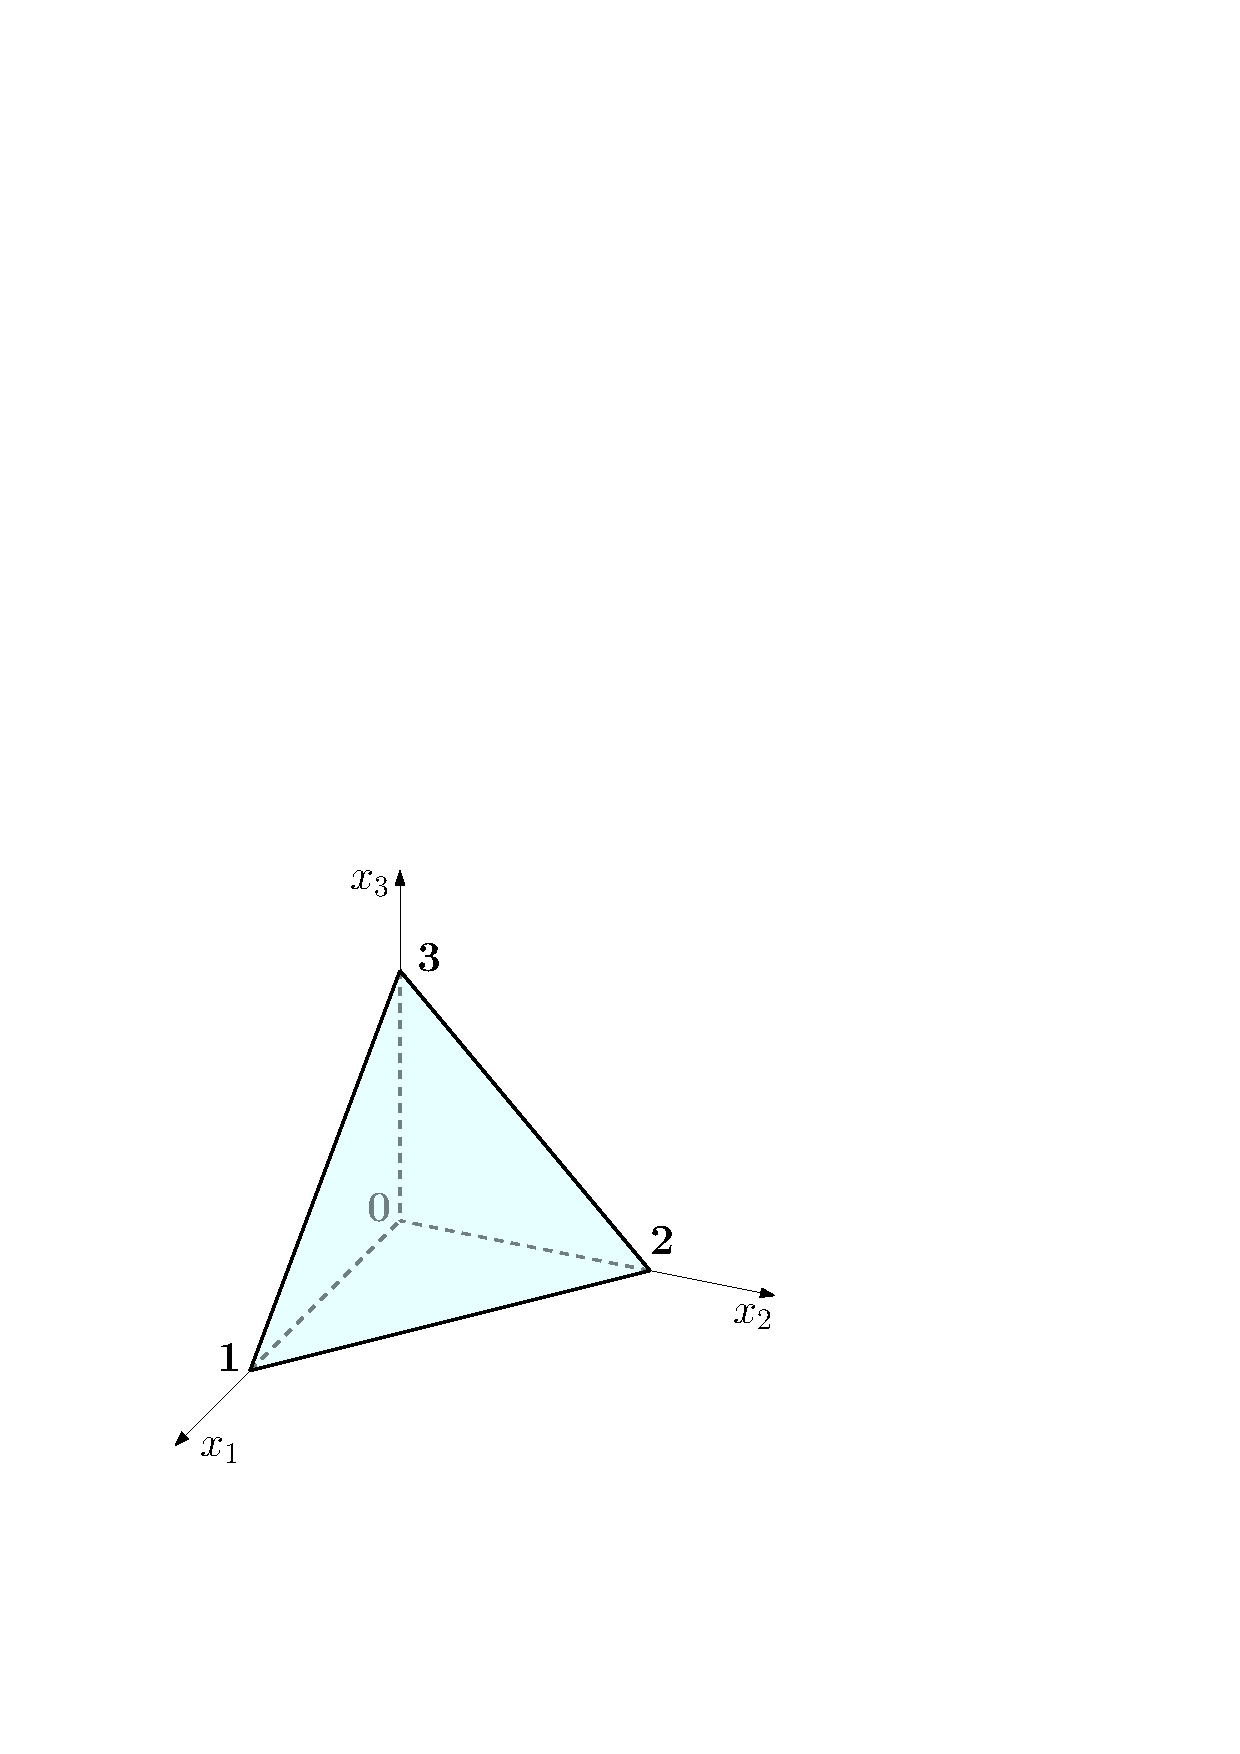
\includegraphics[scale=0.5]{./figures/MasterTet.pdf}
\caption{Master tetrahedron with numbered vertices.}
\label{fig:MasterTet}
\end{center}
\end{figure}

The 3D simplex is the tetrahedron. 
The master element for tetrahedra is illustrated in Figure \ref{fig:MasterTet} in the $x=(x_1,x_2,x_3)$ space.
More precisely, it is the set $\{x\in\R^3:x_1>0,x_2>0,x_3>0,x_1+x_2+x_3<1\}$.
%We shall denote the master tetrahedron by $\hat{\Tri}$ as well, as there will be no confusion with the triangle. The affine coordinates of the tetrahedron will be denoted by $\lambda_0,\lambda_1,\lambda_2,\lambda_3$. By ``edge $0-1$'' we mean the edge defined by $\lambda_0,\lambda_1$ and ``face $0-1-2$'' corresponds to the face defined by $\lambda_0,\lambda_1,\lambda_2$. Observe that
%\be
%\sum_{n=0}^d \lambda_n(x)=1\,,
%\ee
%and
%\be
%\lambda_n(x)\ge0\,,
%\ee
%for all $ x\in\hat\Tri$.

Denote vertex $a$ by $v_a$, so that $v_0=(0,0,0)$, $v_1=(1,0,0)$, $v_2=(0,1,0)$ and $v_3=(0,0,1)$.
As described in \S\ref{sec:affinecoordinates}, the 3D affine coordinates, $\lambda_0$, $\lambda_1$, $\lambda_2$ and $\lambda_3$, are easily calculated for this master tetrahedron:
\begin{equation}
	%\begin{aligned}
	\lambda_0(x)=1-x_1-x_2-x_3\,,\qquad
	\lambda_1(x)=x_1\,,\qquad
	\lambda_2(x)=x_2\,,\qquad
	\lambda_3(x)=x_3\,.
	%\begin{aligned}
\end{equation}
Their gradients are
\begin{equation}
	\nabla\lambda_0(x)=\bigg(\begin{smallmatrix}-1\\[2pt]-1\\[2pt]-1\end{smallmatrix}\bigg)\,,\qquad
	\nabla\lambda_1(x)=\bigg(\begin{smallmatrix}1\\[2pt]0\\[2pt]0\end{smallmatrix}\bigg)\,,\qquad
	\nabla\lambda_2(x)=\bigg(\begin{smallmatrix}0\\[2pt]1\\[2pt]0\end{smallmatrix}\bigg)\,,\qquad
	\nabla\lambda_3(x)=\bigg(\begin{smallmatrix}0\\[2pt]0\\[2pt]1\end{smallmatrix}\bigg)\,.
\end{equation}
These will be used explicitly or implicitly in what follows.

Just like the triangle and the segment, the tetrahedron has a very natural correspondence of its vertices and its affine coordinates.
Quite simply, each vertex $v_a$ is linked to the affine coordinate $\lambda_a$, for $a=0,1,2,3$.
Indeed, $\lambda_a$ takes the value $1$ at the associated vertex.

\subsubsection*{Exact Sequence}

As with the hexahedron, the tetrahedron will have a 3D discrete polynomial exact sequence that represents the continuous exact sequence \eqref{eq:3D_exact_sequence}. 
It is
\begin{equation}
\mathcal{P}^p\,\xrightarrow{\nabla}\,{\mathcal{N}}^p\,\xrightarrow{\nabla\times}\,{\mathcal{RT}}^p\,\xrightarrow{\nabla\cdot}
	\,\mathcal{P}^{p-1} \, ,
\end{equation}
where $\mathcal{P}^p =\mathcal{P}^p(x_1,x_2,x_3)$ is the space of polynomials of total order $p$.
Meanwhile, the N\'{e}d\'{e}lec and Raviart-Thomas spaces for the tetrahedron where already defined by \eqref{eq:NedelecSpace} and \eqref{eq:RaviartThomasSpace}, where $N=3$ in those definitions.

Like the triangle, the tetrahedron sequence has an overall drop in polynomial order of one, which makes it compatible with the construction of the hexahedron.
Also, as noted before, all of the spaces in the exact sequence are invariant under affine transformations. 

%Let $\mathcal{P}^p =\mathcal{P}^p(x_1,x_2,x_3)$ be the space of polynomials of total order $p$ in the $x=(x_1,x_2,x_3)$ space.
%%Define $\mathcal{P}^p = \mathcal{P}^p(\hat\Tri)$ to be the space of polynomials of order $p$ on $\hat\Tri$ and $\left(\mathcal{P}^p\right)^3 = \left(\mathcal{P}^p (\hat\Tri)\right)^3$ to be the triple Cartesian product of $\mathcal{P}^p$ with itself, i.e., vector space of 3-tuples of elements in $\mathcal{P}^p$. Furthermore, define $\tilde{\mathcal{P}}^{p} = \tilde{\mathcal{P}}^{p} (\hat\Tri)$ to be the subspace of homogeneous polynomials of order $p$ on $\hat\Tri$. The space $\left(\tilde{\mathcal{P}}^{p}\right)^d$ is defined similarly.
%%As was the case with the triangle element, it is our intent to reproduce the 3D exact sequence
%Recall the 3D exact sequence
%\begin{equation}
%H^1\,\xrightarrow{\nabla}\,H(\text{curl})\,\xrightarrow{\nabla\times}\,H(\text{div})\,\xrightarrow{\nab\cdot}\,L^2\,.
%\end{equation}
%The corresponding polynomial exact sequence is
%%\be
%%H^1 \, \xrightarrow{\bfnab} \, H(\text{curl}) \, \xrightarrow{\bfnab\times} \, H(\text{div}) \, \xrightarrow{\bfnab\cdot} \, L^2 \, ,
%%\ee
%%at the element level. It is well known that over polynomials, the maximal order exact sequence for the tetrahedron ($d=3$) is
%\begin{equation}
%\mathcal{P}^p\,\xrightarrow{\nabla}\,{\mathcal{N}}^p\,\xrightarrow{\bfnab\times}\,{\mathcal{RT}}^p\,\xrightarrow{\bfnab\cdot}
%	\,\mathcal{P}^{p-1} \, ,
%\end{equation}
%where the definition of the three dimensional N\'{e}d\'{e}lec and Raviart-Thomas spaces, $\mathcal{N}^p$ and $\mathcal{RT}^p$, are reminded next:
%\begin{align}
%	\mathcal{N}^p&=(\mathcal{P}^{p-1})^3\oplus\Big\{E\in(\tilde{\mathcal{P}}^{p})^3: x\cdot E(x)=0\,\text{ for all } 
%		x\in\R^3\Big\}\,,\\
%	\mathcal{RT}^p&=(\mathcal{P}^{p-1})^3\oplus\Big\{V\in(\tilde{\mathcal{P}}^{p})^3:V(x)=\phi(x)x
%		=\phi(x)\Big(\begin{smallmatrix}x_1\\x_2\\x_3\end{smallmatrix}\Big) \, \text{ with }\phi\in\tilde{\mathcal{P}}^{p-1}\Big\}\,.
%\end{align}
%Note the overall drop in polynomial order is one. This makes it compatible with the construction presented for the hexahedron. As before, all of the spaces in the exact sequences above are invariant under affine transformations.

%\be
%{\mathcal{N}}^p := \left(\mathcal{P}^{p-1}\right)^d\oplus\left\{E\in\left(\tilde{\mathcal{P}}^{p}\right)^d \, : \,  x\cdot E( x) = 0 \, \text{ for all }  x\right\} \, ,
%\ee
%and
%\be
%{\mathcal{RT}}^p := \left(\mathcal{P}^{p-1}\right)^d\oplus\left\{V\in\left(\tilde{\mathcal{P}}^{p}\right)^d \, : \,V(x) =  x\,\phi( x) \, \text{ where } \phi \in\tilde{\mathcal{P}}^{p-1}\right\} \, ,
%\ee
%denote the N\'ed\'elec and Raviart-Thomas spaces, respectively.
%\begin{remark}
%As before, all of the spaces in the exact sequences above are invariant under affine transformations. 
%Also, $\Tri$ denotes the tetrahedron in physical space.
%\end{remark}

\subsection{\texorpdfstring{$H^1$}{H1} Shape Functions}
%
%In three dimensions, the trace of $H^1$ functions is the value of the function itself along the boundary.
%Hence, vertex functions should vanish at all nonadjacent faces, edge functions should vanish at all nonadjacent faces, face functions should vanish at all other faces, and bubbles should vanish at all faces.

It will be clear that all the $\frac{1}{6}(p+3)(p+2)(p+1)$ shape functions lie in $\mathcal{P}^{p}$ and span the space.

The ideas in this section are completely parallel to those presented for the triangle (see \S\ref{sec:Tri}) but in three dimensions.
Therefore, the trace properties will not be analyzed in detail, since they follow analogously.

\subsubsection{\texorpdfstring{$H^1$}{H1} Vertices}

%Affine coordinates in three dimensions will be denoted by $\lambda_0$, $\lambda_1$, $\lambda_2$ and $\lambda_3$. They are written explicitly for our master triangle:
%\begin{equation}
%	%\begin{aligned}
%	\lambda_0(x)=1-x_1-x_2-x_3\,,\qquad
%	\lambda_1(x)=x_1\,,\qquad
%	\lambda_2(x)=x_2\,,\qquad
%	\lambda_3(x)=x_3\,.
%	%\begin{aligned}
%\end{equation}
%Their gradients are
%\begin{equation}
%	\nabla\lambda_0(x)=\bigg(\begin{smallmatrix}-1\\[2pt]-1\\[2pt]-1\end{smallmatrix}\bigg)\,,\qquad
%	\nabla\lambda_1(x)=\bigg(\begin{smallmatrix}1\\[2pt]0\\[2pt]0\end{smallmatrix}\bigg)\,,\qquad
%	\nabla\lambda_2(x)=\bigg(\begin{smallmatrix}0\\[2pt]1\\[2pt]0\end{smallmatrix}\bigg)\,,\qquad
%	\nabla\lambda_3(x)=\bigg(\begin{smallmatrix}0\\[2pt]0\\[2pt]1\end{smallmatrix}\bigg)\,.
%\end{equation}
%Take note of the above, since they will be used explicitly or implicitly in the computations of shape functions throughout this section.

%Let $ a_0,\ldots, a_d$, $d=3$, denote the vectices of $\hat\Tri$. Any point $ x\in\hat\Tri$ can be expressed as a convex combination of the vertices,
%\be
% x = \sum_{n=0}^3 \lambda_n a_n\, .
%\ee
%The weight functions, $\lambda_0,\ldots,\lambda_3$, give simplex affine (barycentric, area)coordinates for $\hat\Tri$ and correspond to its vertex shape functions.
%
%In terms of the local coordinates $x_1,x_2,x_3$, we have that
%\begin{equation}
%\begin{array}{ccc}
%\lambda_0(x) &=& 1-x_1-x_2-x_3\\
%\lambda_1(x) &=& x_1\\
%\lambda(x) &=& x_2\\
%\lambda(x) &=& x_3.
%\end{array}
%\end{equation}
%Also, we have
%\begin{equation}\nabla \lambda_0(x) = \left(
%\begin{array}{c}
%-1\\
%-1\\
%-1\\
%\end{array}
%\right),\\ \nabla \lambda_1(x) = \left(
%\begin{array}{c}
%1\\
%0\\
%0\\
%\end{array}
%\right),\\
%\nabla \lambda_2(x) = \left(
%\begin{array}{c}
%0\\
%1\\
%0\\
%\end{array}
%\right),\\
%\nabla \lambda_3(x) = \left(
%\begin{array}{c}
%0\\
%0\\
%1\\
%\end{array}
%\right) \end{equation}

The vertex shape functions and their gradients are simply the affine coordinates themselves,
\begin{equation}
	\phi^\mathrm{v}(x)= \lambda_a(x)\,,\qquad\quad
	\nabla\phi^\mathrm{v}(x)=\nabla\lambda_a(x)\,,
\end{equation}
for $a=0,1,2,3$.
There are a total of $4$ vertex functions (one for each vertex).
%and
%\begin{equation}
%\nabla \phi^\mathrm{v}(x) = %\phi^\vv(s_n(x)) =
%\nabla \lambda_a(x) \, , \quad a=0,1,2,3,
%\label{eq:H1_CountingSimplexVert_tet_2}
%\end{equation}
%where $\nabla \lambda_n(x)$ are as given earlier

%As was the case with the triangular element, we have that the vertex shape functions, being linear functions of the spatial variables, have the required $H^1$ conformity. 
%Again, by construction, the vertex shape functions have the required vanishing properties as well: $\lambda_a(x)$ vanishes at all nodes except node $a$ for $a=0,1,2,3$, and takes the value $1$ at node $a$. They behave linearly, making them compatible with neighbouring elements.

\subsubsection{\texorpdfstring{$H^1$}{H1}  Edges}

These are treated just like triangle edges. 
Hence, one can recur to $\phi_i^\E$ directly. 
Take for instance edge 01. In this case, the shape functions are simply
\begin{equation*}
      \phi_i^\mathrm{e}(x)=\phi_i^\E(\vec{\lambda}_{01}(x))
    	=\underbrace{(\lambda_0(x)+\lambda_1(x))^i}_{\text{blend}}
    		\underbrace{\phi_i^\E\Big(\underbrace{\textstyle{\frac{\lambda_0(x)}{\lambda_0(x)+\lambda_1(x)}},
    			\textstyle{\frac{\lambda_1(x)}{\lambda_0(x)+\lambda_1(x)}}}_{\text{project}}\Big)}_{\text{evaluate}}\,,
\end{equation*}
for $i=2,\ldots,p$. 
%so that $(\tilde{\mu}_0,\tilde{\mu}_1)=(\frac{\lambda_0}{\lambda_0+\lambda_1},\frac{\lambda_1}{\lambda_0+\lambda_1})$ are the projected 1D affine coordinates. Since $\tilde{\mu}_1(x)=\frac{x_1}{1-x_2-x_3}$, this implies there is a three dimensional projection of the form 
The projection being implied is
\begin{equation*}
	(x_1,x_2,x_3)\;\longmapsto\;(\textstyle{\frac{x_1}{1-x_3}},\textstyle{\frac{x_2}{1-x_3}},0)
		\;\longmapsto\;(\textstyle{\frac{x_1}{1-x_2-x_3}},0,0)\,.
\end{equation*}
It consists of finding the intersection $P''=(\frac{x_1}{1-x_2-x_3},0,0)$ of the edge with the projecting plane passing through the original point $P=(x_1,x_2,x_3)$ and the opposite nonadjacent edge.
It is illustrated in Figure \ref{fig:TetProjection}. 
Alternatively it can be interpreted in two steps.
First it is projected to a point $P'$ in an adjacent face, using the projecting line passing through $P$ and the disjoint vertex to the face.
Once in the face, it is projected again to the desired edge using the traditional \textit{two} dimensional triangle projection (see Figure \ref{fig:TriangleProjection}).

\begin{figure}[!ht]
\begin{center}
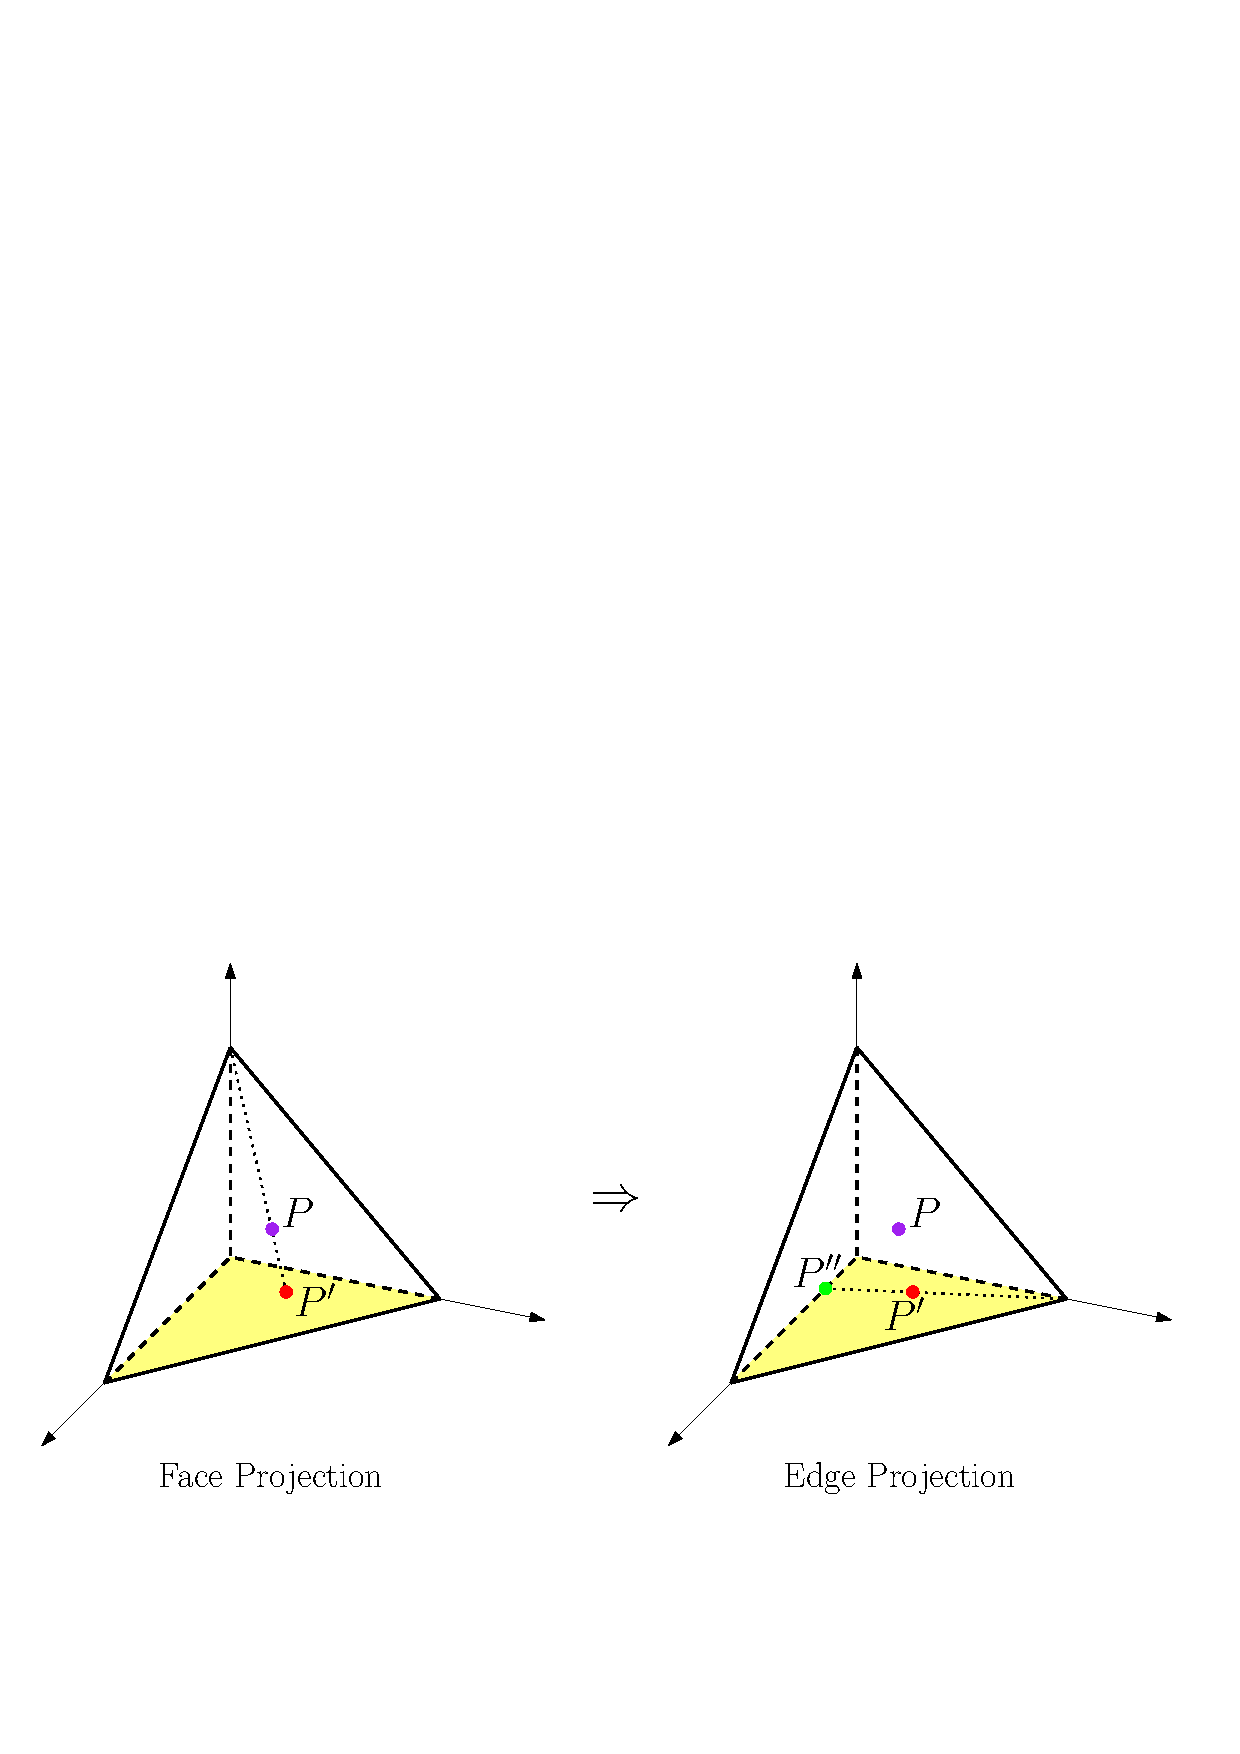
\includegraphics[scale=0.6]{./figures/TetProjection.pdf}
\caption{Face projection from $P$ to $P'$ followed by an edge projection from $P'$ to $P''$.}
\label{fig:TetProjection}
\end{center}
\end{figure}

More generally, the edge functions and their gradients are
\begin{equation}
	\phi_i^\mathrm{e}(x)=\phi_i^\E(\vec{\lambda}_{ab}(x))\,,\qquad\quad
		\nabla\phi_i^\mathrm{e}(x)=\nabla\phi_i^\E(\vec{\lambda}_{ab}(x))\,,
	\label{eq:Tetphigeneral}
\end{equation}
with $i=2,\ldots,p$, $0\leq a<b\leq3$. 
There are a total of $p-1$ edge functions for every given edge, leading to a total of $6(p-1)$ edge functions.

%For simplicity, we first consider the $0-1$ edge. Also, we consider the orientation $\oo=0$ case initially. As was the case with the triangular element, the map that associates a point in the tetrahedron the corresponding point on the edge with edge coordinates:
%\be
%\mu_n = \frac{\lambda_n}{\lambda_0+\lambda_1},\quad n=0,1\, ,
%\ee
%can be viewed as a projection onto the edge, whereas function
%$(\lambda_0 + \lambda_1)^i$ is the edge blending function.
%
%\begin{figure}[ht!]
%    \centering
%   % \begin{subfigure}[b]{0.45\textwidth}
%    %    \includegraphics[width=\textwidth]{./tri_V2.png}
%    %    \caption{Edge $H^1$ bubble for the triangle.}
%     %   \label{fig:H1edgebub_tri}
%    %\end{subfigure}%
%    ~ %add desired spacing between images, e. g. ~, \quad, \qquad, \hfill etc.
%      %(or a blank line to force the subfigure onto a new line)
%    \begin{subfigure}[b]{0.45\textwidth}
%        \includegraphics[width=\textwidth]{./figures/tet_V2.png}
%        \caption{Edge $H^1$ bubble projection for the tet.}
%    \end{subfigure}
%    \caption{Edge shape functions.}\label{fig:H1edgebub_tet}
%% \label{fig:H1bub_tri}
%\end{figure}

%We thus see that the edge function corresponding to the $0-1$ edge is $L_i(\lambda_1;\lambda_0+\lambda_1)$

%It follows from the construction that  $\phi^\E_i(\lambda_0,\lambda_1)$ satisfies the required vanishing property. Indeed, by construction, $\phi^\E_i(\lambda_0,\lambda_1)$ is nonzero on the $0-1$ edge and zero on the other two edges. Also, 
%\begin{equation}
%\phi^{\e,\oo}_i(\lambda_0,\lambda_1) = \nabla \phi^\E_i(\lambda_0,\lambda_1)
%\nonumber
%\end{equation}
% lies in the proper N\'ed\'elec space.


%With the above definition, we find that the $H^1$ edge shape functions are composed of the shape functions above, i.e., $\phi^\E_i$, considered on each edge independently;
%\be
%\phi^\mathrm{e}_i(x) = \phi^{\e}_i(\lambda_a(x),\lambda_b(x))% = \left[L_i\right](s_k,s_l)
% \, , \quad i=2,\ldots,p\, , \quad k<l=0,\ldots,3\,.
%\label{eq:H1_CountingSimplexEdge}
%\ee

%\paragraph{Edge Orientations}
%These are dealt with analogously to the triangular edge orientations as explained before. 
%This also applies to $H(\mathrm{curl})$ oriented edge shape functions.
%In order to incorporate the orientation embedding into the shape functions constructed in the above discussion, we modify the equations as follows (again, considering the $0-1$ edge as an example):
%\be
%\phi^{\e,\oo}_i(\lambda_0,\lambda_1) =
%\left\{
%    \begin{array}{ll}
%        \left[L_i\right](\lambda_0,\lambda_1) = L_i(\lambda_1;\lambda_0+\lambda_1) & \text{if } \oo = 0\\
%        \left[L_i\right](\lambda_1,\lambda_0) = L_i(\lambda_0;\lambda_1+\lambda_1) & \text{if } \oo = 1
%    \end{array}
%\right.
%\ee
% For simplicity, we have assumed unswapped coordinates in each case above.

% We leave it as a simple excercise for the reader to show that if we allow for $i=1$ in the definiton~\eqref{eq:H1_CountingSimplexEdge}, then $\phi_1(s_k,s_l)$ agrees with the vertex shape functions defined previously, albeit with some overcounting in the case of the tetrahedron.
% \textcolor{red}{Provide pictorial illustration of the projection in
% both 2D and 3D.}


% \textcolor{red}{Provide a pictorial example in 2D for an edge shape function}

\subsubsection{\texorpdfstring{$H^1$}{H1} Faces}

The construction of these shape functions follows simply by homogenizing the $H^1$ triangle face bubbles, since this will represent a polynomial extension preserving the desired vanishing properties.
This explains the definition of $\phi_{ij}^\Tri$ in terms of homogenized polynomials.
As an example, consider face 012, where the shape functions are
%In general, homogenization is the ideal tool to construct extensions for simplicial geometries
%To construct these shape functions, consider an $H^1$ triangle face bubble restricted to one face of the tetrahedron. For instance, take face 012, which corresponds to $\lambda_3=0$. Here, we already know the restriction of our shape function, which should be $\phi_{ij}^\Tri$. Homogenizing produces an $(i+j)$ order polynomial extension preserving the vanishing property on all other faces:
\begin{equation*}
	\phi_{ij}^\mathrm{f}(x)=\phi_{ij}^\Tri(\vec{\lambda}_{012}(x))=
		\underbrace{(\lambda_0(x)+\lambda_1(x)+\lambda_2(x))^{i+j}}_{\text{blend}}\underbrace{\phi_{ij}^\Tri
			\Big(\underbrace{\textstyle{\frac{1}{\lambda_0(x)+\lambda_1(x)+\lambda_2(x)}}
				\vec{\lambda}_{012}(x)}_{\text{project}}\Big)}_{\text{evaluate}}\,,
%	\phi_{ij}^\Tri(\lambda_0,\lambda_1,\lambda_2)=[L_i,L_j^{2i}](\lambda_0,\lambda_1,\lambda_2)
%		=(\lambda_0+\lambda_1+\lambda_2)^{i+j}[L_i,L_j^{2i}]
%			(\textstyle{\frac{\lambda_0}{\lambda_0+\lambda_1+\lambda_2}},\textstyle{\frac{\lambda_1}{\lambda_0+\lambda_1+\lambda_2}}
%				,\textstyle{\frac{\lambda_2}{\lambda_0+\lambda_1+\lambda_2}})\,.
\end{equation*}
for $i\geq2$ and $j\geq1$.
%Here, $(\tilde{\nu}_0,\tilde{\nu}_1,\tilde{\nu}_2)=(\frac{\lambda_0}{\lambda_0+\lambda_1+\lambda_2}, \frac{\lambda_1}{\lambda_0+\lambda_1+\lambda_2}, \frac{\lambda_2}{\lambda_0+\lambda_1+\lambda_2})$, are the projected two dimensional affine coordinates. 
%The projection is already illustrated in Figure \ref{fig:TetProjection} and has the form
%\begin{equation*}
%	(x_1,x_2,x_3)\;\longmapsto\;(\textstyle{\frac{x_1}{1-x_3}},\textstyle{\frac{x_2}{1-x_3}},0)\,.
%\end{equation*}
The projection is already illustrated in Figure \ref{fig:TetProjection} and consists of finding the intersection $P'=(\frac{x_1}{1-x_3},\frac{x_2}{1-x_3},0)$ of the face with the projecting line passing through the original point $P=(x_1,x_2,x_3)$ and the opposite vertex to the face. 
%This is illustrated in Figure \textit{add Figure}.

The full collection of shape functions and their gradient is
\begin{equation}
	\phi_{ij}^\mathrm{f}(x)=\phi_{ij}^\Tri(\vec{\lambda}_{abc}(x))\,,\qquad\quad
			\nabla\phi_{ij}^\mathrm{f}(x)=\nabla\phi_{ij}^\Tri(\vec{\lambda}_{abc}(x))\,,
			\label{eq:H1Tetfaces}
\end{equation}
where $i\geq2$, $j\ge1$, $n=i+j=3,\ldots,p$, and $0\leq a<b<c\leq3$. 
There are $\frac{1}{2}(p-1)(p-2)$ shape functions for each face, leading to a total of $2(p-1)(p-2)$ face functions.
%Homogenizing produces an $(i+j)$-order polynomial extension preserving the vanishing property on all other faces;
%\be
%\begin{array}{ll}
%\phi^\f_{ij}(\lambda_0,\lambda_1,\lambda_2) & = L_i\left(
%\frac{\frac{\lambda_1}{\lambda_0 + \lambda_1 + \lambda_2}}
%{\frac{\lambda_0}{\lambda_0 + \lambda_1 + \lambda_2}
%+\frac{\lambda_1}{\lambda_0 + \lambda_1 + \lambda_2}} \right)
%\left(
%\frac{\lambda_0 + \lambda_1}{\lambda_0 + \lambda_1 + \lambda_2} \right)^i
%L^{2i-1}_{j} \left(\frac{\lambda_2}{\lambda_0 + \lambda_1 + \lambda_2}\right)
%(\lambda_0 + \lambda_1 + \lambda_2)^{i+j} \\[20pt]
%& = L_i(\lambda_1; \lambda_0 + \lambda_1) L^{2i-1}_{j} (\lambda_2;
%\lambda_0 + \lambda_1 + \lambda_2)\\[12pt]
%& = \left[L_i,L^{2i-1}_{j}\right] (\lambda_0,\lambda_1,\lambda_2)\, .
%\end{array}
%\label{H1_TetHomog}
%\ee

%To construct the entire set of tetrahedron face bubbles, we must consider each face independently and so form the collection of shape functions
%\be
%\phi^\mathrm{f}_{ij}(x) = \phi^{\f}_{ij}(\lambda_a(x),\lambda_b(x),\lambda_c(x))% = \left[L_i,L^{2i-1}_{j}\right] (\lambda_k,\lambda_l,\lambda_m)\, ,%
%% \quad i\ge2,\, j\ge1, \, i+j=3,\ldots,p\, , \quad k<l<m=0,\ldots,3\,.
%\label{eq:H1_CountingTetFace}
%\ee
%% \be
%% \left\{\phi(x)\in\mathcal{P}^p(\hat\Tri) : \phi(x) = \phi^\f_{ij}(\lambda_k(x),\lambda_l(x),\lambda_m(x))\right\}
%% % \quad i\ge2,\, j\ge1, \, i+j=3,\ldots,p\, , \quad k<l<m=0,\ldots,3
%% \,,
%% \label{eq:H1_CountingTetFace}
%% \ee
%here, the indices range $i\ge2,\, j\ge1,\, i+j \leq p$, and $a\leq b \leq c \in\{0,1,2,3\}$.


%\paragraph{Face Orientations.}
%To consider orientations, simply take a predefined $\oo=0$ orientation for a given triangular face, and replace $\phi_{ij}^\Tri$ with $\phi_{ij}^{\Tri,\oo}$ (and similarly with the gradients). For instance, take face 123, which has a predefined local numbering of the vertices symbolized by $\xi^\mathrm{f}$ which goes from vertex 1 to vertex 2 to vertex 3. This defines the $\oo=0$ orientation and determines the order in which the entries should go in $\phi_{ij}^{\Tri,\oo}$. This way, for face 012, \eqref{eq:H1Tetfaces} becomes
%\begin{equation*}
%	\phi_{ij}^\mathrm{f}(x)=\phi_{ij}^{\Tri,\oo}(\lambda_1(x),\lambda_2(x),\lambda_3(x))\,,
%\end{equation*}
%with $i\geq2$, $j\ge1$, $n=i+j=3,\ldots,p$. The entries are then permuted according to orientation $\oo$ as described in \S\ref{sec:TriaFaceOrientations}. For this example, if $\oo=3$, it takes the form 
%\begin{equation*}
%	\phi_{ij}^\mathrm{f}(x)=\phi_{ij}^{\Tri,3}(\lambda_1(x),\lambda_2(x),\lambda_3(x))
%		=\phi_{ij}^\Tri(\lambda_1(x),\lambda_3(x),\lambda_2(x))\,,
%\end{equation*}
%with $i\geq2$, $j\ge1$, $n=i+j=3,\ldots,p$.

%To account for orientation embeddings, refer the reader to the permutation table defining $\sigma_{mathrm{o}}(\cdot)$ in the triangle section. With the permutation functions $\sigma_\oo$, $\oo=0,\ldots,5$ given in Figure~\ref{table:functionSigma}, we can fully define the affine $H^1$ face shape function for the $\lambda_3=0$ face of the tetrahedron
%\be
%\phi^{\f,\oo}_{ij}(\lambda_0,\lambda_1,\lambda_2) = \left[L_i,L^{2i-1}_{j}\right] (\lambda_{\sigma_\oo(0)},\lambda_{\sigma_\oo(1)},\lambda_{\sigma_\oo(2)})\,,
%\ee
%where $\oo=0,\ldots5$ denotes the given orientation of the affine coordinate system. The affine $H^1$ face shape function for all other faces are similarly defined.


\subsubsection{\texorpdfstring{$H^1$}{H1} Interior Bubbles}

The tetrahedron bubbles are given by blending a face shape function with a polynomial of complementing order which vanishes on the remaining face. 
As with triangles, it is carefully chosen as a Jacobi polynomial $L_k^{2(i+j)}$. 

The interior functions and their gradient are
\begin{equation}
	\begin{aligned}
		\phi_{ijk}^\mathrm{b}(x)&=\phi_{ij}^\Tri(\vec{\lambda}_{012}(x))[L_k^{2(i+j)}](\vec{\mu}_{01}(\lambda_3(x)))\,,\\
			\nabla\phi_{ijk}^\mathrm{b}(x)&=[L_k^{2(i+j)}](\vec{\mu}_{01}(\lambda_3(x)))\nabla\phi_{ij}^\Tri(\vec{\lambda}_{012}(x))
				+\phi_{ij}^\Tri(\vec{\lambda}_{012}(x))\nabla[L_k^{2(i+j)}](\vec{\mu}_{01}(\lambda_3(x)))\,,
	\end{aligned}
\end{equation}
%\begin{equation}
%\phi^\bb_{ijk}(\lambda_0,\lambda_1,\lambda_2,\lambda_3)
%&=  \phi^\f_{ij} (\lambda_0,\lambda_1,\lambda_2) \, \hat\phi_k(\lambda_3)
%\nonumber\\
%&= L_i(\lambda_1;\lambda_0+\lambda_1) L^{2i-1}_{j}
%(\lambda_2;\lambda_0+\lambda_1+\lambda_2) L^{2(i+j)-1}_{k} (\lambda_3)
%\nonumber\\
%&= \left[L_i,L^{2i-1}_{j},L^{2(i+j)-1}_{k}\right](\lambda_0,\lambda_1,\lambda_2,\lambda_3)
%\label{eq:H1_TetBubb}
%\end{equation}
where $i\geq2$, $j\geq1$, $k\geq1$ and $n=i+j+k=4,\ldots,p$, and where $\vec{\mu}_{01}(\lambda_3(x))=(1-\lambda_3(x),\lambda_3(x))$.
%Their gradients are
%\begin{equation}
%	\nabla\phi_{ijk}^\mathrm{b}(x)=L_k^{2(i+j)}(\lambda_3(x))\nabla\phi_{ij}^\Tri(\lambda_0(x),\lambda_1(x),\lambda_2(x))
%		+\phi_{ij}^\Tri(\lambda_0(x),\lambda_1(x),\lambda_2(x))P_{k-1}^{2(i+j)}(\lambda_3(x))\nabla\lambda_3(x)\,.
%\end{equation}
There are $\frac{1}{6}(p-1)(p-2)(p-3)$ interior shape functions in total.



%
%$$
%i \ge 2,\, j \ge 1,\, k \ge 1,\, i+j+k \leq p.
%$$ In the final line of Equation~\eqref{eq:H1_TetBubb}, we have used the property \mbox{$\sum\limits_{n=0}^3 \lambda_n = 1$}.
%
%The $H^1$ tetrahedron bubbles are defined
%\be
%\phi^\mathrm{b}_{ijk}(x) = \phi^\bb_{ijk}(\lambda_0(x),\lambda_1(x),\lambda_2(x),\lambda_3(x))\, ,
%\quad i \ge 2,\, j \ge 1,\, k \ge 1,\, i+j+k \leq p \, ,
%\label{eq:H1_CountingTetBubb}
%\ee
%for all $x\in\hat\Tri$.
%%
%\paragraph{\texorpdfstring{$H^1$}{H1} Linear Independence}
%
%To account for all of the constructed shape functions for the tetrahedron, we set $d=3$ and sum Equations~\eqref{eq:H1_CountingSimplexVert}, \eqref{eq:H1_CountingSimplexEdge}, \eqref{eq:H1_CountingTetFace}, \eqref{eq:H1_CountingTetBubb}. Accounting for the 4 vertices, 6 edges, and 4 faces, we have constructed
%\be
%4+6(p-1)+4{p-1\choose 2}+{p-1\choose 3} = {p+3\choose 3}
%\ee
%shape functions. Note that ${p+3\choose 3}$ is also the dimension of the polynomial space $\mathcal{P}^p$ in $\mathbb{R}^3$.
%
%The linear independence of the above shape functions, using the presented Lobatto and integrated Jacobi polynomials is given in \textit{cite Beuchler} and \textit{cite}.
%
%Since the cardinality of our set of linearly independent shape functions agrees with the dimension of $\mathcal{P}^p$ for the tetrahedron, we understand that our set is spanning and that we have constructed an appropriate basis for the space.

\subsection{\texorpdfstring{$H(\mathrm{curl})$}{Hcurl} Shape Functions}

%In three dimensions, the trace of $H(\mathrm{curl})$ functions is the tangential component of the vector function along the boundary.
%All edge functions should have vanishing trace at all other edges, and all face functions should have vanishing trace at all other faces, while the bubbles should have zero trace along all faces.

The dimension of $\mathcal{N}^p$ in three dimensions is $\frac{1}{2}p(p+2)(p+3)$.
A careful count of the linearly independent shape functions to be presented throughout this section will coincide with that dimension. 
Showing that the functions constructed are in $\mathcal{N}^p$ follows from Lemma \ref{lemma:curl}.
The constructions are all analogous to those of the triangle and simply require of an extra extension which is naturally provided by homogenization.
%We ask the reader to review the corresponding section of the triangle element. The constructions are all analogous and simply require of an extra extension which is naturally provided by homogenization.
%In particular, we shall be using the lemmata stated in that section for the $H(\text{curl})$ shape functions for the tetrahedron.

\subsubsection{\texorpdfstring{$H(\mathrm{curl})$}{Hcurl} Edges}

%Consider the $0-1$ edge of a tetrahedron. Here again, we no longer need an endpoint vanishing property for the edge shape functions. Without taking into account embedded orienations, for an edge with endpoint affine coordinates $0-1$, we define the affine $H(\text{curl})$ edge functions by:
%\be
%E^\E_i(\lambda_0,\lambda_1) = \left[\hat\psi_i\right](\lambda_0,\lambda_1)
%(\lambda_0 \bfnab \lambda_1 - \lambda_1 \bfnab \lambda_0 )\, , \quad i=0,\ldots,p-1\,.
%\label{eq:edge_curl_25}
%\ee
%If $\hat\psi_i = P_i$, where $P_i$ denotes the shifted scaled Legendre polynomial of order $i$, then clearly, $$\left[\hat\psi_i\right] = \left[P_i\right]\,,$$ and by Lemma~\ref{lemma:curl},
%\be
%\bfnab \times E_i^\E(\lambda_0,\lambda_1) =  (i+2) \, \left[P_i\right](\lambda_0,\lambda_1) \,
%\bfnab \lambda_0 \times \bfnab \lambda_1 \, .
%\ee
%
%The complete collection of $H(\text{curl})$ edge shape functions is generated by
%\be
%E^\mathrm{e}_i(x) = E_i^{\e}(\lambda_a(x),\lambda_b(x)), \quad i\leq p\,,
%\ee
%where we account for all edges by considering all $0\leq a \leq b\leq 3$.

%\paragraph{Orientation Considerations}
%Taking into account orientation changes on the edge, as before we have the following orientation embedded definitions for the affine $H(\text{curl})$ edge functions:
%\be
%E^{\e,\oo}_i(\lambda_0,\lambda_1) =
%\left\{
%    \begin{array}{ll}
%        \left[P_i\right](\lambda_0,\lambda_1)\left(\lambda_0 \bfnab \lambda_1 - \lambda_1 \bfnab \lambda_0\right) & \text{if } \oo =0 \\
%        \left[P_i\right](\lambda_1,\lambda_0)\left(\lambda_1 \bfnab \lambda_0 - \lambda_0 \bfnab \lambda_1\right) & \text{if } \oo =1
%    \end{array}
%\right.
%\ee

These are just the same as in the triangle case, but using three dimensional affine coordinates for the homogenization.
For example, for edge 01, the shape functions are
\begin{equation*}
	\begin{aligned}
		E_i^\mathrm{e}(x)&=E_i^\E(\vec{\lambda}_{01}(x))=
			[P_i](\vec{\lambda}_{01}(x))\Big(\lambda_0(x)\nabla\lambda_1(x)-\lambda_1(x)\nabla\lambda_0(x)\Big)\\
    	&=(\lambda_0(x)+\lambda_1(x))^i
    [P_i]\Big(\textstyle{\frac{\lambda_0(x)}{\lambda_0(x)+\lambda_1(x)}},\textstyle{\frac{\lambda_1(x)}{\lambda_0(x)+\lambda_1(x)}}\Big)
    			E_0^\E(\vec{\lambda}_{01}(x))\\
    	&=\underbrace{(\lambda_0(x)+\lambda_1(x))^{i+2}}_{\text{blend}}
    		\underbrace{E_i^\E\Big(\underbrace{\textstyle{\frac{\lambda_0(x)}{\lambda_0(x)+\lambda_1(x)}},
    			\textstyle{\frac{\lambda_1(x)}{\lambda_0(x)+\lambda_1(x)}}}_{\text{project}}\Big)}_{\text{evaluate}}\,,
	\end{aligned}
\end{equation*}
for $i=0,\ldots,p-1$.
Regarding the traces, note that they are completely inherited from $E_0^\E(\vec{\lambda}_{01}(x))$, which is a Whitney function known to have the desired vanishing properties and being tracewise compatible with the lower dimensional triangle edge functions.
Therefore, all trace properties are satisfied, including the nonzero decay along the adjacent faces to the edge.

The edge functions with their curl are
\begin{equation}
	E_i^\mathrm{e}(x)=E_i^\E(\vec{\lambda}_{ab}(x))\,,\qquad\quad
		\nabla\times E_i^\mathrm{e}(x)=\nabla\times E_i^\E(\vec{\lambda}_{ab}(x))\,,
	\label{eq:TetEgeneral}
\end{equation}
for $i=0,\ldots,p-1$, and $0\leq a<b\leq3$. 
There are a total of $p$ edge functions for every given edge, for a total of $6p$ edge functions.

\subsubsection{\texorpdfstring{$H(\mathrm{curl})$}{Hcurl} Faces}

%Take $p$ to be the order of $\lambda_3=0$ face of the tetrahedron and take $i \geq 0,\, j \geq 1,\, i+j\leq p-1$. Assume that we have orientation $\oo=0$ on this face. Recall the construction of the triangle $H(\text{curl})$ bubbles: $E^{\Tri\text{ ,I}}_{ij}(s_0(x),s_1(x),s_2(x))$ and $E^{\Tri\text{ ,II}}_{ij}(s_0(x),s_1(x),s_2(x))$. Introducing $s_i=\lambda_i, \text{ } i = 0,1,2,3,$ we arrive at the $H(\text{curl})$ tetrahedron face functions.

%Collecting all of the $H(\text{curl})$ tetrahedron face functions together, we have two families accounting for each of the four faces ($a,b,c = 0,1,2,3, \text{ }0 \leq a \leq b \leq c \leq 3$):
%\begin{description}
%  \item[Family I:]
%\be
%E^\mathrm{f}_{ij}(x) = E^{\f, \text{ I}}_{ij}(\lambda_a(x),\lambda_b(x),\lambda_c(x)),\quad i \geq 0,\, j \geq 1,\quad i+j=1,\ldots,p-1
%\ee
%
%  \item[Family II:]
%\be
%E^\mathrm{f}_{ij}(x) = E^{\f,\text{ II}}_{ij}(\lambda_a(x),\lambda_b(x),\lambda_c(x)),\quad i \geq 0,\, j \geq 1,\quad i+j=1,\ldots,p-1\,.
%\ee
%\end{description}

Like the triangle, the tetrahedron has two families of shape functions for every face.
The trace properties follow from those of the edge functions.
There is a grand total of $4p(p-1)$ face functions.

\subparagraph{Family I:} 
The shape functions and their curls are
\begin{equation}
	E_{ij}^{\mathrm{f}}(x)=E_{ij}^\Tri(\vec{\lambda}_{abc}(x))\,,\qquad\quad
		\nabla\times E_{ij}^{\mathrm{f}}(x)=\nabla\times E_{ij}^\Tri(\vec{\lambda}_{abc}(x))\,,
\end{equation}
for $i\geq0$, $j\geq1$, $n=i+j=1,\ldots,p-1$, and $0\leq a<b<c\leq3$. 
For every face, there are $\frac{1}{2}p(p-1)$ face functions in this family.

\subparagraph{Family II:}
The shape functions and their curls are
\begin{equation}
	E_{ij}^{\mathrm{f}}(x)=E_{ij}^\Tri(\vec{\lambda}_{bca}(x))\,,\qquad\quad
		\nabla\times E_{ij}^{\mathrm{f}}(x)=\nabla\times E_{ij}^\Tri(\vec{\lambda}_{bca}(x))\,,
\end{equation}
for $i\geq0$, $j\geq1$, $n=i+j=1,\ldots,p-1$, and $0\leq a<b<c\leq3$.
The only difference with the first family is that the entries are permuted to $\vec{\lambda}_{bca}(x)$ instead of $\vec{\lambda}_{abc}(x)$.
For every face, there are $\frac{1}{2}p(p-1)$ face functions in this family.

%\paragraph{Orientation Considerations}
%
%Accounting for orientations, we define the first family of orientated affine $H(\text{curl})$ tetrahedron face functions on the $\lambda_3=0$ face
%\be
%E^{\f,\oo}_{ij}(\lambda_0,\lambda_1,\lambda_2) = \left[P_i,L^{2i-1}_{j}\right](\lambda_{\sigma_\oo(0)},\lambda_{\sigma_\oo(1)},\lambda_{\sigma_\oo(2)})\left(\lambda_{\sigma_\oo(0)} \bfnab \lambda_{\sigma_\oo(1)} - \lambda_{\sigma_\oo(1)} \bfnab \lambda_{\sigma_\oo(0)}\right)\,.
%\ee
%The second family is obtained by rotating the affine coordinates one index, i.e. setting:
%$$
%\lambda_i := \lambda_{i+1},\quad i=0,1,2
%$$
%where $i+1 := \text{mod}(i+1,2)$.


\subsubsection{\texorpdfstring{$H(\mathrm{curl})$}{Hcurl} Interior Bubbles}

%As with $H^1$ bubbles these are obtained by blending a face shape function in $H(\mathrm{curl})$ with a polynomial of complementing order which vanishes on the remaining face. It is chosen as the Jacobi polynomial $L_k^{2(i+j)}$. Here, one must be careful about double counting. The bubbles are

The construction is completely analogous to that of $H^1$ in the sense that they are obtained by multiplying the face functions by the Jacobi polynomial $L_k^{2(i+j)}$.
One must attempt this for various possible permutations of the entries, but being careful to ensure that they are linearly independent.
Three families arise.

The interior bubbles and their curl are
\begin{equation}
	\begin{aligned}
		E_{ijk}^\mathrm{b}(x)&=[L_k^{2(i+j)}](\vec{\mu}_{01}(\lambda_d(x)))E_{ij}^\Tri(\vec{\lambda}_{abc}(x))\,,\\
		\nabla\!\!\times\! E_{ijk}^\mathrm{b}(x)&=[L_k^{2(i+j)}](\vec{\mu}_{01}(\lambda_d(x)))
			\nabla\!\!\times\! E_{ij}^\Tri(\vec{\lambda}_{abc}(x))
				\!+\!\nabla[L_k^{2(i+j)}](\vec{\mu}_{01}(\lambda_d(x)))\!\times\! E_{ij}^\Tri(\vec{\lambda}_{abc}(x))\,,
	\end{aligned}
\end{equation}
where $i\geq0$, $j\geq1$, $k\geq1$, $n=i+j+k=2,\ldots,p-1$ and $(a,b,c,d)=(0,1,2,3),(1,2,3,0),(2,3,0,1)$, and where $\vec{\mu}_{01}(\lambda_d(x))=(1-\lambda_d(x),\lambda_d(x))$.
There is a grand total of $\frac{1}{2}p(p-1)(p-2)$ interior shape functions.

%\begin{equation}
%	E_{ijk}^\mathrm{b}(x)=E_{ij}^{\Tri_I}(\lambda_a(x),\lambda_b(x),\lambda_c(x))L_k^{2(i+j)}(\lambda_d(x))\,,
%\end{equation}
% Their curls are
%\begin{equation}
%	\nabla\times E_{ijk}^\mathrm{b}(x)=L_k^{2(i+j)}(\lambda_d(x))\nabla\times E_{ij}^{\Tri_I}(\lambda_a(x),\lambda_b(x),\lambda_c(x))
%		+P_{k-1}^{2(i+j)}\nabla\lambda_d(x)\times E_{ij}^{\Tri_I}(\lambda_a(x),\lambda_b(x),\lambda_c(x))\,.
%\end{equation}


%Let $p$ be the order of $H^1$ element's middle node and take $i\geq 0,j\ge 1,\, k\ge 1,\, i+j+k=2,\ldots,p-1$. The construction of the $H(\text{curl})$ tetrahedron bubbles is similar as to has been seen previously in the other bubble functions. Since we need not worry about orientations, the first family of shape functions of order $i+j+k$, is simply given by:
%\be
%E^\mathrm{b}_{ijk}(x) = E^\bb_{ijk}(\lambda_0(x),\lambda_1(x),\lambda_2(x),\lambda_3(x)),
%\ee
%where
%\begin{align}
%E^\bb_{ijk}(\lambda_0,\lambda_1,\lambda_2,\lambda_3) &= E^\f_{ij}(\lambda_0,\lambda_1,\lambda_2)\,L^{2(i+j)-1}_{k}(\lambda_3)
%\nonumber\\
%& = \left[P_i,L^{2i-1}_{j},L^{2(i+j)-1}_{k}\right](\lambda_0,\lambda_1,\lambda_2,\lambda_3) (\lambda_0 \bfnab \lambda_1 - \lambda_1 \bfnab \lambda_0)\,.
%\end{align}
%
%Observe that the curl is readily computed
%\be
%\begin{array}{rl}
%\bfnab \times E^\bb_{ijk} & = \bfnab \times E^\f_{ij} (\lambda_0,\lambda_1,\lambda_2)\, L^{2(i+j)-1}_{k}(\lambda_3) + E^\f_{ij}(\lambda_0,\lambda_1,\lambda_2) \times \bfnab L^{2(i+j)-1}_{k}(\lambda_3)\\
%&= \bfnab \times E^\f_{ij} (\lambda_0,\lambda_1,\lambda_2)\, L^{2(i+j)-1}_{k}(\lambda_3)\\
%&\quad + \left[P_i,L^{2i-1}_j,P^{2(i+j)-1}_{k-1}\right](\lambda_0,\lambda_1,\lambda_2,\lambda_3)\,\left(\lambda_0 \bfnab \lambda_1 - \lambda_1 \bfnab \lambda_0\right)\times\bfnab\lambda_3\,.
%\end{array}
%\ee
%
%The second family and third families are obtained by rotating the affine coordinates, as we see in the following forumlas:
%\begin{description}
%  \item[Family I:]
%\be
%E^\mathrm{b}_{ijk}(x) = E^\bb_{ijk}(\lambda_0(x),\lambda_1(x),\lambda_2(x),\lambda_3(x)),\quad i\geq 0,j\ge 1,\, k\ge 1 \quad i+j+k=2,\ldots,p-1
%\ee
%
%  \item[Family II:]
%\be
%E^\mathrm{b}_{ijk}(x) = E^\bb_{ijk}(\lambda_1(x),\lambda_2(x),\lambda_3(x),\lambda_0(x)),\quad i\geq 0,j\ge 1,\, k\ge 1 \quad i+j+k=2,\ldots,p-1
%\ee
%
%  \item[Family III:]
%\be
%E^\mathrm{b}_{ijk}(x) = E^\bb_{ijk}(\lambda_2(x),\lambda_3(x),\lambda_0(x),\lambda_1(x)),\quad i\geq 0,j\ge 1,\, k\ge 1 \quad i+j+k=2,\ldots,p-1\,.
%\ee
%\end{description}



%\paragraph{\boldmath{$H(\text{curl})$} Linear Independence}
%
%Note that for the tetrahedron we have constructed
%\be
%6p+8{p\choose2}+3{p\choose3} = \frac{p(p+2)(p+3)}{2}
%\ee
%shape functions.


\subsection{\texorpdfstring{$H(\mathrm{div})$}{Hdiv} Shape Functions}

%In three dimensions, the trace of $H(\mathrm{div})$ functions is the tangential component of the vector function along the boundary.
%All face functions should have vanishing trace at all other faces, while the bubbles should have zero trace at all faces. 

The dimension of $\mathcal{RT}^p$ in three dimensions is $\frac{1}{2}p(p+1)(p+3)$.
A careful count of the linearly independent shape functions presented here will coincide with that dimension. 
Showing that the functions constructed are in $\mathcal{RT}^p$ is not immediate, but follows from the next lemma, which should be kept in mind.

\begin{lemma}
\label{lemma:div}
Let $x\in\R^N$ for $N=3$, and $f_n\in\mathcal{P}^n(x)$ be any polynomial of total order $n$ in the coordinates $x=(x_1,x_2,x_3)$. Given $s_0$, $s_1$ and $s_2$ affine coordinates in $\R^3$ $($or simply linear functions in $x$$)$, it follows that the Raviart-Thomas space of order $n+1$, $\mathcal{RT}^{n+1}$, contains the function 
\begin{equation*}
	f_n(\bcdot)\Big(s_0\nabla s_1\times\nabla s_2+s_1\nabla s_2\times\nabla s_0+s_2\nabla s_0\times\nabla s_1\Big)\in\mathcal{RT}^{n+1}\,.
\end{equation*}
\end{lemma}
\begin{proof}
Recall the definition of the Raviart-Thomas space in three dimensions,
\begin{equation*}
	\mathcal{RT}^p=(\mathcal{P}^{p-1})^3\oplus\Big\{V\in(\tilde{\mathcal{P}}^{p})^3:V(x)=\phi(x)x
		=\phi(x)\Big(\begin{smallmatrix}x_1\\x_2\\x_3\end{smallmatrix}\Big) \, \text{ with }\phi\in\tilde{\mathcal{P}}^{p-1}\Big\}\,.
\end{equation*}
Affine coordinates are linear functions in $x=(x_1,x_2,x_3)$, so that
\begin{equation*}
	s_k(x)=a_k+b_k\cdot x\,,
\end{equation*}
for $a_k\in\R$, $b_k\in\R^3$ and $k=0,1,2$. Then $\nabla s_k(x)=b_k$ and
\begin{align*}
	V(x)&=s_0(x)\nabla s_1(x)\times\nabla s_2(x)+s_1(x)\nabla s_2(x)\times\nabla s_0(x)+s_2(x)\nabla s_0(x)\times\nabla s_1(x)\\
		&=(a_0+b_0\cdot x)(b_1\times b_2)+(a_1+b_1\cdot x)(b_2\times b_0)+(a_2+b_2\cdot x)(b_0\times b_1)\\
		&=\underbrace{\Big(a_0(b_1\times b_2)+a_1(b_2\times b_0)+a_2(b_0\times b_1)\Big)}_{=A}
			+\underbrace{\Big(b_0\cdot(b_1\times b_2)\Big)x}_{=B(x)}\,,			
\end{align*}
where the last term follows from various identities. Clearly, $A\in(\mathcal{P}^0)^3=\R^3$ and $b_0\cdot(b_1\times b_2)\in\tilde{\mathcal{P}}^0=\R$, so that $B\in\{V\in(\tilde{\mathcal{P}}^{1})^3: V(x)=\phi(x)x\}$. Hence, $V\in\mathcal{RT}^1$.

Now, $f_n\in\mathcal{P}^n=\mathcal{P}^{n-1}\oplus\tilde{\mathcal{P}}^n$, for $n\geq1$ can always be decoupled into $f_n=f_{n-1}+\tilde{f}_n$, where $f_{n-1}\in\mathcal{P}^{n-1}$ and $\tilde{f}_n\in\tilde{\mathcal{P}}^n$. As a result
\begin{equation*}
	f_n(x)V(x)=f_n(x)A+f_{n-1}(x)B(x)+\tilde{f}_n(x)B(x)\,,
\end{equation*}
where it is clear $f_{n}A+f_{n-1}B\in(\mathcal{P}^n)^3$ and $\tilde{f}_nB\in\{V\in(\tilde{\mathcal{P}}^{n+1})^3: V(x)=\phi(x)x\}$. Therefore, $f_nV\in\mathcal{RT}^{n+1}$.
\end{proof}
%As with the previous section on $H(\text{curl})$ shape functions, we begin with a lemma.

%\begin{lemma}
%\label{lemma:div}
%Let $V$ be a vector-valued function defined on a tetrahedron, given by:
%\be
%V =
%f_n(\lambda_0,\lambda_1,\lambda_2)
%\,
%[\lambda_0 \, \bfnab \lambda_1 \times \bfnab \lambda_2 +
%\lambda_1 \, \bfnab \lambda_2 \times \bfnab \lambda_0 +
%\lambda_2 \, \bfnab \lambda_0 \times \bfnab \lambda_1 ]
%\ee
%where $\lambda_0,\lambda_1, \lambda_2$ are differentiable functions of the spatial coordinates, and $f_n(t_1,t_2,t_3)$ is a
%homogeneous polynomial of (total) order $n$ in $t_1,t_2,t_3$. Then,
%\be
%\bfnab \cdot V = (n+3) \,
%f_n(\lambda_0,\lambda_1,\lambda_2)
%\, (\bfnab \lambda_0 \times \bfnab \lambda_1) \cdot \bfnab \lambda_2 \, .
%\ee
%Moreover, if $\lambda_0,\lambda_1, \lambda_2$ are affine coordinates, then $V$ belongs to the Raviart-Thomas space of order $n$,
%\be
%V \in \mathcal{RT}^n% := \left\{  x\phi( x) \, : \, \phi \in\tilde{\mathcal{P}}^{n-1}\right\}.
%.
%\ee
%\end{lemma}
%\begin{proof}
%Let us assume
%\be
%f_n(\lambda_0,\lambda_1) = g_n\left(\frac{\lambda_0}{\lambda_0+\lambda_1+\lambda_2},\frac{\lambda_1}{\lambda_0+\lambda_1+\lambda_2},\frac{\lambda_2}{\lambda_0+\lambda_1+\lambda_2}\right)\left(\lambda_0+\lambda_1+\lambda_2\right)^n
%\ee
%for some differentiable function, $g_n\in\mathcal{P}^n$.
%
%Here, we see that
%\begin{align*}
%\bfnab \cdot V &= \bfnab \cdot f_n(\lambda_0,\lambda_1,\lambda_2)
%\,
%[\lambda_0 \, \bfnab \lambda_1 \times \bfnab \lambda_2 +
%\lambda_1 \, \bfnab \lambda_2 \times \bfnab \lambda_0 +
%\lambda_2 \, \bfnab \lambda_0 \times \bfnab \lambda_1 ]\\
%&= \bfnab \left( g_n\left(\frac{\lambda_0}{\lambda_0+\lambda_1+\lambda_2},\frac{\lambda_1}{\lambda_0+\lambda_1+\lambda_2},\frac{\lambda_2}{\lambda_0+\lambda_1+\lambda_2}\right)\left(\lambda_0+\lambda_1+\lambda_2\right)^n\right)\\
%&\quad \cdot \,
%[\lambda_0 \, \bfnab \lambda_1 \times \bfnab \lambda_2 +
%\lambda_1 \, \bfnab \lambda_2 \times \bfnab \lambda_0 +
%\lambda_2 \, \bfnab \lambda_0 \times \bfnab \lambda_1 ]\\
%&\quad + f_n(\lambda_0,\lambda_1,\lambda_2) \, \bfnab \cdot \,
%[\lambda_0 \, \bfnab \lambda_1 \times \bfnab \lambda_2 +
%\lambda_1 \, \bfnab \lambda_2 \times \bfnab \lambda_0 +
%\lambda_2 \, \bfnab \lambda_0 \times \bfnab \lambda_1 ]\\
%&= \bfnab g_n\left(\frac{\lambda_0}{\lambda_0+\lambda_1+\lambda_2},\frac{\lambda_1}{\lambda_0+\lambda_1+\lambda_2},\frac{\lambda_2}{\lambda_0+\lambda_1+\lambda_2}\right)\left(\lambda_0+\lambda_1+\lambda_2\right)^n\\
%&\quad \cdot \,
%[\lambda_0 \, \bfnab \lambda_1 \times \bfnab \lambda_2 +
%\lambda_1 \, \bfnab \lambda_2 \times \bfnab \lambda_0 +
%\lambda_2 \, \bfnab \lambda_0 \times \bfnab \lambda_1 ]\\
%&\quad + n f_n(\lambda_0,\lambda_1,\lambda_2)\left(\bfnab\lambda_0+\bfnab\lambda_1+\bfnab\lambda_2\right)\left(\lambda_0+\lambda_1+\lambda_2\right)^{-1}\\
%&\quad \cdot \,
%[\lambda_0 \, \bfnab \lambda_1 \times \bfnab \lambda_2 +
%\lambda_1 \, \bfnab \lambda_2 \times \bfnab \lambda_0 +
%\lambda_2 \, \bfnab \lambda_0 \times \bfnab \lambda_1 ]\\
%&\quad + 3f_n(\lambda_0,\lambda_1,\lambda_2) \, (\bfnab \lambda_0 \times \bfnab \lambda_1) \cdot \bfnab \lambda_2\\
%&= (n+3)\,f_n(\lambda_0,\lambda_1,\lambda_2) \, (\bfnab \lambda_0 \times \bfnab \lambda_1) \cdot \bfnab \lambda_2,
%\end{align*}
%since
%\be
%\bfnab g_n\left(\frac{\lambda_0}{\lambda_0+\lambda_1+\lambda_2},\frac{\lambda_1}{\lambda_0+\lambda_1+\lambda_2},\frac{\lambda_2}{\lambda_0+\lambda_1+\lambda_2}\right) \quad \perp  \quad [\lambda_0 \, \bfnab \lambda_1 \times \bfnab \lambda_2 +
%\lambda_1 \, \bfnab \lambda_2 \times \bfnab \lambda_0 +
%\lambda_2 \, \bfnab \lambda_0 \times \bfnab \lambda_1 ].
%\ee
%
%Now, let $ x = (x_1,x_2,x_3)$ be the Cartesian coordinates of $ x\in\hat\Tri$, $\{\bfe_i\}_{i=1}^3$ be the Euclidean basis for $\mathbb{R}^3$, and $\eps_{ijk}$, for $i,j,k=1,2,3$, be the Levi-Civita tensor in $\mathbb{R}^3$,. Then, with
%\be
%\lambda_m = a_m + \sum_{i=1}^3 b_{mi}x_i,
%\ee
%where $a_m,b_{mi}\in\mathbb{R}$, $m=1,2$, $i=1,2,3$ we find that
%\begin{align*}
%&\quad \lambda_0 \, \bfnab \lambda_1 \times \bfnab \lambda_2 +
%\lambda_1 \, \bfnab \lambda_2 \times \bfnab \lambda_0 +
%\lambda_2 \, \bfnab \lambda_0 \times \bfnab \lambda_1\\
%&=  \sum_{i,j,k=1}^3\eps_{ijk}\left(a_0b_{1j}b_{2k}+a_1b_{2j}b_{0k}+a_2b_{0j}b_{1k}\right)\bfe_i + \sum_{i,j,k,l=1}^3\eps_{ijk}\left(b_{0l}b_{1j}b_{2k}+b_{1l}b_{2j}b_{0k}+b_{2l}b_{0j}b_{1k}\right)x_l\bfe_i\\
%&=  \sum_{i,j,k=1}^3\eps_{ijk}\left(a_0b_{1j}b_{2k}+a_1b_{2j}b_{0k}+a_2b_{0j}b_{1k}\right)\bfe_i + \sum_{i,j,k=1}^3\eps_{ijk}\left(b_{0i}b_{1j}b_{2k}+b_{1i}b_{2j}b_{0k}+b_{2i}b_{0j}b_{1k}\right)x_i\bfe_i,
%\end{align*}
%where the final line follows from symmetries of $\eps_{ijk}$.
%
%This completes the proof of Lemma 2.
%
%\end{proof}


\subsubsection{\texorpdfstring{$H(\mathrm{div})$}{Hdiv} Faces}
%As we have done throughout the previous discussion of the tetrahedral element, we consider the face $\lambda_3=0$ with orienation $0$. The affine $H(\text{div})$ face shape functions are:
%\be
%V^\f_{ij}(\lambda_0,\lambda_1,\lambda_2) = \left[P_i,P^{2i-1}_j\right](\lambda_0,\lambda_1,\lambda_2)
%\left( \lambda_0\,  \bfnab \lambda_1 \times \bfnab \lambda_2 +
%       \lambda_1\,  \bfnab \lambda_2 \times \bfnab \lambda_0 +
%       \lambda_2\,  \bfnab \lambda_0 \times \bfnab \lambda_1 \right)
%\label{eq:face_div}
%\ee
%with
%$$
%i\geq 0,\, j\ge 0,\quad i+j=0,\ldots,p-1\,,
%$$
%where $p$ is the face order for the corresponding $H^1$ element.
%As was the case with triangle $H(\text{curl})$ face functions, we can use the above formula for $V^\f_{ij}(\lambda_0,\lambda_1,\lambda_2)$ as a motivation for the following, more general definition.

The general formula for these functions is motivated by the well known first order Whitney form for $H(\mathrm{div})$, along with the fact that the normal trace of the faces should span the two dimensional $L^2$ space. The general definition is presented next.

\begin{definition*}
Let $s_0$, $s_1$ and $s_2$ be arbitrary functions of some spatial variable in $\R^N$, with $N=3$, and denote by $p$ the order in the coordinate triplet $(s_0,s_1,s_2)$. Then
\begin{equation}
	V_{ij}^{\Tri}(s_0,s_1,s_2)=[P_i,P_j^{2i+1}](s_0,s_1,s_2)\Big(s_0\nabla s_1\times\nabla s_2
		+s_1\nabla s_2\times\nabla s_0+s_2\nabla s_0\times\nabla s_1\Big)\,,
\end{equation}
for $i=n-j$, $j=0,\ldots,n$ and $n=0,\ldots,p-1$ $($or equivalently $i\geq0$, $j\geq0$ and $n=i+j=0,\ldots,p-1$$)$. The divergence is
\begin{equation}
	\nabla\cdot V_{ij}^{\Tri}(s_0,s_1,s_2)=(i+j+3)[P_i,P_j^{2i+1}](s_0,s_1,s_2)\nabla s_0\cdot(\nabla s_1\times\nabla s_2) \,.
	\label{eq:VdeltaDiv}
\end{equation}
\end{definition*}

The formula for the divergence follows from the following lemma, because $[P_i,P_j^{2i+1}](s_0,s_1,s_2)$ is a homogeneous polynomial of total order $n=i+j$ in $s_0$, $s_1$ and $s_2$.

\begin{lemma}
\label{lem:divformula}
Let $\psi_n(s_0,s_1,s_2)\in\tilde{\mathcal{P}}^n(s_0,s_1,s_2)$ be a homogeneous polynomial of total order $n$ in $s_0$, $s_1$ and $s_2$, where $s_0$, $s_1$ and $s_2$ are arbitrary functions of some spatial variable in $\R^N$, with $N=3$. Then
\begin{equation*}
    \nabla\cdot\Big(\psi_n(s_0,s_1,s_2)(s_0\nabla s_1\times\nabla s_2
			+s_1\nabla s_2\times\nabla s_0+s_2\nabla s_0\times\nabla s_1)\Big)
				\!=\!(n+3)\psi_n(s_0,s_1,s_2)\nabla s_0\cdot(\nabla s_1\times\nabla s_2)\,.
\end{equation*}
\end{lemma}
\begin{proof}
Let $V_{00}^{\Tri}(s_0,s_1,s_2)=(s_0\nabla s_1\times\nabla s_2
			+s_1\nabla s_2\times\nabla s_0+s_2\nabla s_0\times\nabla s_1)$. First notice that
\begin{align*}
	\nabla\cdot \Big(s_0(\nabla s_1\times\nabla s_2)\Big)
		&=\nabla s_0\cdot(\nabla s_1\times\nabla s_2)
			+s_0\Big(\nabla s_2\cdot\nabla\times\nabla s_1-\nabla s_1\cdot\nabla\times\nabla s_2\Big)\\
		&=\nabla s_0\cdot(\nabla s_1\times\nabla s_2)\,,
\end{align*}
and similarly with $\nabla\cdot(s_1(\nabla s_2\times\nabla s_0))$ and $\nabla\cdot(s_2(\nabla s_1\times\nabla s_2))$. All of them result in a scalar triple product, which is invariant to cyclic permutations. It follows
\begin{equation*}
	\nabla\cdot V_{00}^{\Tri}(s_0,s_1,s_2)=3\nabla s_0\cdot(\nabla s_1\times\nabla s_2)\,.
\end{equation*}
Now, consider a monomial $s_0^as_1^bs_2^c$. Then
\begin{align*}
	\nabla(s_0^as_1^bs_2^c)\cdot V_{00}^{\Tri}(s_0,s_1,s_2)
		&=(as_0^{a-1}s_1^bs_2^c\nabla s_0+bs_0^as_1^{b-1}s_2^c\nabla s_1+cs_0^as_1^bs_2^{c-1}\nabla s_2)
			\cdot V_{00}^{\Tri}(s_0,s_1,s_2)\\
		&=as_0^{a-1}s_1^bs_2^cs_0\nabla s_0\cdot(\nabla s_1\times\nabla s_2)
			+bs_0^as_1^{b-1}s_2^cs_1\nabla s_1\cdot(\nabla s_2\times\nabla s_0)\\
				&\qquad\qquad\qquad\qquad\qquad\qquad\qquad\qquad+cs_0^as_1^bs_2^{c-1}s_2\nabla s_2\cdot(\nabla s_0\times\nabla s_1)\\
		&=(a+b+c)s_0^as_1^bs_2^c\nabla s_0\cdot(\nabla s_1\times\nabla s_2)\,.
\end{align*}
With these last two results it follows
\begin{equation*}
	\nabla\cdot\Big(s_0^as_1^bs_2^cV_{00}^{\Tri}(s_0,s_1,s_2)\Big)=(a+b+c+3)s_0^as_1^bs_2^c\nabla s_0\cdot(\nabla s_1\times\nabla s_2)\,.
\end{equation*}
Then observe that any homogeneous polynomial $\psi_n(s_0,s_1,s_2)$ is composed of monomials of the form $s_0^as_1^bs_2^c$ of \textit{fixed} total order $a+b+c=n$. The result immediately follows.
\end{proof}

The result in \eqref{eq:VdeltaDiv} is quite remarkable in the sense that, as required by the construction, there are no derivatives of $[P_i,P_j^{2i+1}](s_0,s_1,s_2)$ in the expression for the divergence. 
Although not used in this section, record the following useful remark which will be exploited when dealing with the prism and pyramid elements.
\begin{remark}
Let $\nu_0=1-\nu_1-\nu_2$, where $\nu_1$ and $\nu_2$ are arbitrary functions of some spatial variable in $\R^N$ with $N=3$, and where $p$ is the order in the coordinates $(\nu_0,\nu_1,\nu_2)$. Then for all $i\geq0$, $j\geq0$ and $n=i+j=0,\ldots,p-1$,
\begin{equation}
    V_{ij}^\Tri(\nu_0,\nu_1,\nu_2)=[P_i,P_j^{2i+1}](\nu_0,\nu_1,\nu_2)\nabla\nu_1\times\nabla\nu_2\,,
    	\quad\qquad \nabla\cdot V_{ij}^\Tri(\nu_0,\nu_1,\nu_2)=0\,.\label{eq:HdivtriangleRemark}
\end{equation}
\end{remark}

These functions are still represented by the same projection, and follow the logic of projecting, evaluating and blending.
For example, take face 012, so the shape functions are
\begin{equation*}
	V_{ij}^\mathrm{f}(x)=V_{ij}^\Tri(\vec{\lambda}_{012}(x))=
		\underbrace{(\lambda_0(x)+\lambda_1(x)+\lambda_2(x))^{i+j+3}}_{\text{blend}}\underbrace{V_{ij}^\Tri
			\Big(\underbrace{\textstyle{\frac{1}{\lambda_0(x)+\lambda_1(x)+\lambda_2(x)}}
				\vec{\lambda}_{012}(x)}_{\text{project}}\Big)}_{\text{evaluate}}\,,
\end{equation*}
for $i\geq0$ and $j\geq0$.
It can be readily checked that they satisfy the required vanishing properties by focusing on the lowest order function $V_{00}^\mathrm{f}(x)$.
Moreover, by Lemma \ref{lemma:div} it is clear $V_{ij}^\mathrm{f}\in\mathcal{RT}^{n+1}$ for $n=i+j$. 

More generally, the shape functions and their divergence are
\begin{equation}
	V_{ij}^\mathrm{f}(x)=V_{ij}^\Tri(\vec{\lambda}_{abc}(x))\,,\qquad\quad
		\nabla\cdot V_{ij}^\mathrm{f}(x)=\nabla \cdot V_{ij}^\Tri(\vec{\lambda}_{abc}(x))\,,
\end{equation}
where $i\geq0$, $j\geq0$, $n=i+j=0,\ldots,p-1$, and $0\leq a<b<c\leq3$. 
%It can be readily checked they satisfy the required vanishing properties, and by Lemma \ref{lemma:div} it is clear $V_{ij}^\mathrm{f}\in\mathcal{RT}^{n+1}$ for $n=i+j$. 
Clearly, for each face there are $\frac{1}{2}p(p+1)$ functions, giving a total of $2p(p+1)$ face functions.
%\begin{definition*} Given the bubble function $V^\f_{ij}(s_0(x),s_1(x),s_2(x))$ with arguments $s_0(x),s_1(x),s_2(x)$, the corresponding two sets of $H(\text{div})$ triangle bubbles are: \\$V^{\f, \text{ I}}_{ij}(s_0(x),s_1(x),s_2(x)) = V^\f_{ij}(s_0(x),s_1(x),s_2(x)) \\
%V^{\f, \text{ II}}_{ij}(s_0(x),s_1(x),s_2(x)) = V^\f_{ij}(s_1(x),s_2(x),s_0(x))$ \\
%where \be
%V^\f_{ij}(s_0,s_1,s_2) = \left[P_i,P^{2i-1}_j\right](s_0,s_1,s_2)
%\left( s_0\,  \bfnab s_1 \times \bfnab s_2 +
%       s_1\,  \bfnab s_2 \times \bfnab s_0 +
%       s_2\,  \bfnab s_0 \times \bfnab s_1 \right)
%\label{eq:face_div_1}
%\nonumber
%\ee
%\\\end{definition*}
% One may observe that restricted to this face, the normal component of $V^\f_{ij}$ reduces to:
% $$
% V^\f_{ij} \cdot n_f = \left[P_i\right](\lambda_0,\lambda_1) \, P^{2i-1}_j(\lambda_2) \, .
% $$
% If we introduce:
% $$
% f_n(\lambda_0,\lambda_1,\lambda_2) =
% \left[P_i\right](\lambda_0,\lambda_1) \, P^{2i-1}_j(\lambda_2) \, ,
% $$
% the relation between the homogenized polynomials and scaled Legendre polynomials is
% $$
% [f]_n(\lambda_0,\lambda_1,\lambda_2)
% = \left[P_i,P^{2i-1}_j\right] (\lambda_0,\lambda_1,\lambda_2) .
% $$
%Specializing the above formula for the case of affine coordinates ($s_i=\lambda_i$, $i=0,1,2,3$), we now collect the families of $H(\text{div})$ face shape functions for each face,
%\begin{description}
%  \item[Family I:]
%\be
%V^\mathrm{f}_{ij}(x) = V^{\f,\text{ I}}_{ij}(\lambda_a(x),\lambda_b(x),\lambda_c(x)),\quad i \geq 0,\, j \geq 0,\quad i+j=0,\ldots,p-1
%\ee
%
%  \item[Family II:]
%\be
%V^\mathrm{f}_{ij}(x) = V^{\f,\text{ II}}_{ij}(\lambda_a(x),\lambda_b(x),\lambda_c(x)),\quad i \geq 0,\, j \geq 0,\quad i+j=0,\ldots,p-1\,.
%\ee
%\end{description}
%
%Moreover, by Lemma~\ref{lemma:div},
%\be
%\bfnab \cdot V^{\f,\text{ I}}_{ij}(\lambda_0,\lambda_1,\lambda_2) = (i+j+3) \left[P_i,P^{2i-1}_j\right] (\lambda_0,\lambda_1,\lambda_2)
%\, (\bfnab \lambda_0 \times \bfnab \lambda_1) \cdot \bfnab \lambda_2 \, ,
%\ee
%is easily computed, and lies in the correct energy space. Similar calculations hold for $V^{\f,\text{ II}}_{ij}(\cdot,\cdot,\cdot)$.

%\paragraph{Orientation Considerations}
%
%We now consider orientation embedded face functions. Defining
%\[
%V^\f_{00}(\lambda_0,\lambda_1,\lambda_2) = \left( \lambda_0\,  \bfnab \lambda_1 \times \bfnab \lambda_2 +
%       \lambda_1\,  \bfnab \lambda_2 \times \bfnab \lambda_0 +
%       \lambda_2\,  \bfnab \lambda_0 \times \bfnab \lambda_1 \right)\,,
%\]
%we can easily define the oriented affine $H(\text{div})$ face shape functions for the $\lambda_3=0$ face,
%\be
%V^{\f,\oo}_{ij}(\lambda_0,\lambda_1,\lambda_2) = \left[P_i,P^{2i-1}_j\right](\lambda_{\sigma_\oo(0)},\lambda_{\sigma_\oo(1)},\lambda_{\sigma_\oo(2)})\,V^\f_{00}(\lambda_{\sigma_\oo(0)},\lambda_{\sigma_\oo(1)},\lambda_{\sigma_\oo(2)})\,,
%\ee
%where $\sigma_\oo$ is the permutation of indices defined in Table~\ref{table:functionSigma}, $\oo=0,\ldots,5$. Similar definitions follow for the other faces.

\subsubsection{\texorpdfstring{$H(\mathrm{div})$}{Hdiv} Interior Bubbles}

%These are obtained by taking the $H(\mathrm{div})$ face functions and combining them with a polynomial of complementing order which vanishes on the remaining face. 
The construction is just like in $H^1$ and $H(\mathrm{curl})$, and there are three resulting families to consider.
The polynomial chosen to vanish is the Jacobi polynomial, $L_k^{2(i+j+1)}$. 

The interior functions with their divergence are
\begin{equation}
	\begin{aligned}
		V_{ijk}^\mathrm{b}(x)&=[L_k^{2(i\!+\!j\!+\!1)}](\vec{\mu}_{01}(\lambda_d(x)))V_{ij}^\Tri(\vec{\lambda}_{abc}(x))\,,\\
		\nabla\!\!\cdot\! V_{ijk}^\mathrm{b}(x)&=[L_k^{2(i\!+\!j\!+\!1)}](\vec{\mu}_{01}(\lambda_d(x)))
			\nabla\!\!\cdot\! V_{ij}^\Tri(\vec{\lambda}_{abc}(x))
				\!+\!\nabla[L_k^{2(i\!+\!j\!+\!1)}](\vec{\mu}_{01}(\lambda_d(x)))\!\cdot\! V_{ij}^\Tri(\vec{\lambda}_{abc}(x))\,,
	\end{aligned}
\end{equation}
where $i\geq0$, $j\geq0$, $k\geq1$, $n=i+j+k=1,\ldots,p-1$ and $(a,b,c,d)=(0,1,2,3),(1,2,3,0),(2,3,0,1)$, and where $\vec{\mu}_{01}(\lambda_d(x))=(1-\lambda_d(x),\lambda_d(x))$.
%Their divergence is
%\begin{equation}
%	\nabla\cdot V_{ijk}^\mathrm{b}(x)=L_k^{2(i+j+1)}(\lambda_d(x))\nabla\cdot V_{ij}^{\Tri}(\lambda_a(x),\lambda_b(x),\lambda_c(x))
%		+P_{k-1}^{2(i+j+1)}\nabla\lambda_d(x)\cdot V_{ij}^{\Tri}(\lambda_a(x),\lambda_b(x),\lambda_c(x))\,.
%\end{equation}
There is a grand total of $\frac{1}{2}p(p-1)(p+1)$ interior shape functions.

%No longer needing to worry about orienations, we define three families of affine $H(\text{div})$ tetrahedron bubbles on the $\lambda_3=0$ face. Let $p$ be the order of the exact sequence and $i,j\geq 0,\, k \geq 1,\,i+j+k=1,\ldots,p-1$, then the first family is defined as follows:
%\begin{align}
%V^\bb_{ijk}(\lambda_0,\lambda_1,\lambda_2,\lambda_3) &= V^\f_{ij} (\lambda_0,\lambda_1,\lambda_2)\, L^{2(i+j)-1}_k(\lambda_3)\\
%&= \left[P_i,P_j^{2i-1},L^{2(i+j)-1}_k\right](\lambda_0,\lambda_1,\lambda_2,\lambda_3) V^\f_{00}(\lambda_0,\lambda_1,\lambda_2,\lambda_3)\,,
%\end{align}
%where $V^f_{ij}$ is the affine face shape vector-valued polynomial
%of order $i+j$ defined by \textit{reference}, and $L^{\alpha}_k$ is the integrated scaled Jacobi polynomial of order $k$ and weight $2(i+j)-1$.
%
%The corresponding divergence is easily computed
%\begin{align}
%\bfnab \cdot V^\bb_{ijk}(\lambda_0,\lambda_1,\lambda_2,\lambda_3) &= \bfnab \cdot V^\f_{ij} (\lambda_0,\lambda_1,\lambda_2)\, L^{2(i+j)-1}_k(\lambda_3)
%+ V^\f_{ij} (\lambda_0,\lambda_1,\lambda_2)\cdot P^{2(i+j)-1}_{k-1} (\lambda_3) \bfnab \lambda_3
%\nonumber\\
%&= \left((i+j+3)L^{2(i+j)-1}_k(\lambda_3) -(\lambda_0+\lambda_1+\lambda_2)P^{2(i+j)-1}_{k-1} (\lambda_3)\right)
%\nonumber\\
%&\quad+\left[P_i,P^{2i-1}_j\right](\lambda_0,\lambda_1,\lambda_2) (\bfnab \lambda_0 \times \bfnab \lambda_1) \cdot \bfnab \lambda_2
%\end{align}
%The next two families are defined by rotating affine coordinates.
%
%\begin{description}
%  \item[Family I:]
%\be
%V^\mathrm{b}_{ijk}(x) = V^\bb_{ijk}(\lambda_0(x),\lambda_1(x),\lambda_2(x),\lambda_3(x)),\quad i\geq 0,j\ge 0,\, k\ge 1 \quad i+j+k=1,\ldots,p-1
%\ee
%
%  \item[Family II:]
%\be
%V^\mathrm{b}_{ijk}(x) = V^\bb_{ijk}(\lambda_1(x),\lambda_2(x),\lambda_3(x),\lambda_0(x)),\quad i\geq 0,j\ge 0,\, k\ge 1 \quad i+j+k=1,\ldots,p-1
%\ee
%
%  \item[Family III:]
%\be
%V^\mathrm{b}_{ijk}(x) = V^\bb_{ijk}(\lambda_2(x),\lambda_3(x),\lambda_0(x),\lambda_1(x)),\quad i\geq 0,j\ge 0,\, k\ge 1 \quad i+j+k=1,\ldots,p-1\,.
%\ee
%
%\end{description}
%

%\paragraph{\boldmath{$H(\text{div})$} Linear Independence}
%
%% Note that for the triangle, the map
%% \be
%% \varphi(x,y)=(y,-x),
%% \ee
%% is bijective from ${\mathop\mathcal{P}\limits_\sim}^{p-1}\oplus{\mathop\mathcal{N}\limits_\sim}^p$ to ${\mathop\mathcal{P}\limits_\sim}^{p-1}\oplus{\mathop\mathcal{T}\limits_\sim}^p$ and so we need not consider $H(\text{div})$ for the triangle.
%
%For the tetrahedron we have constructed
%\be
%4{p+1\choose2}+3{p+1\choose3} = \frac{p(p+1)(p+3)}{2}
%\ee
%shape functions.

\subsection{\texorpdfstring{$L^2$}{L2} Shape Functions}
The $\frac{1}{6}p(p+2)(p+1)$ shape functions will clearly span $\mathcal{P}^{p-1}$.

\subsubsection{\texorpdfstring{$L^2$}{L2} Interior}

Similar to the construction of $L^2$ triangle functions, the $L^2$ interior functions for the tetrahedron are
\begin{equation}
	\begin{aligned}
		\psi_{ijk}^\mathrm{b}(x)&=[P_i](\lambda_0(x),\lambda_1(x))[P_j^{2i+1}](\lambda_0(x)\!+\!\lambda_1(x),\lambda_2(x))
			[P_k^{2(i+j+1)}](1\!-\!\lambda_3(x),\lambda_3(x))\\
		&=[P_i,P_j^{2i+1}](\vec{\lambda}_{012}(x))[P_k^{2(i+j+1)}](\vec{\mu}_{01}(\lambda_3(x)))
			(\nabla\lambda_1(x)\!\!\times\!\!\nabla\lambda_2(x))\!\cdot\!\nabla\lambda_3(x)\,,
	\end{aligned}
\end{equation}
where $i\geq0$, $j\geq0$, $k\geq0$, and $n=i+j+k=0,\ldots,p-1$, and where $\vec{\mu}_{01}(\lambda_3(x))=(1-\lambda_3(x),\lambda_3(x))$. There is a total of $\frac{1}{6}p(p+2)(p+1)$ interior functions.
%$$
%i,j,k \geq 0,\quad i+j+k=0,\ldots,p-1 \, .
%$$

%\paragraph{\texorpdfstring{$L^2$}{L2} Linear Independence}
%
%We clearly have
%\be
%{p+2\choose3}
%\ee
%shape functions for the tetrahedron.
%
%The verification that we have constructed a basis follows similarly from the $H^1$ case.

\subsection{Orientations}
\label{sec:TetOrientations}

\begin{figure}[!ht]
\begin{center}
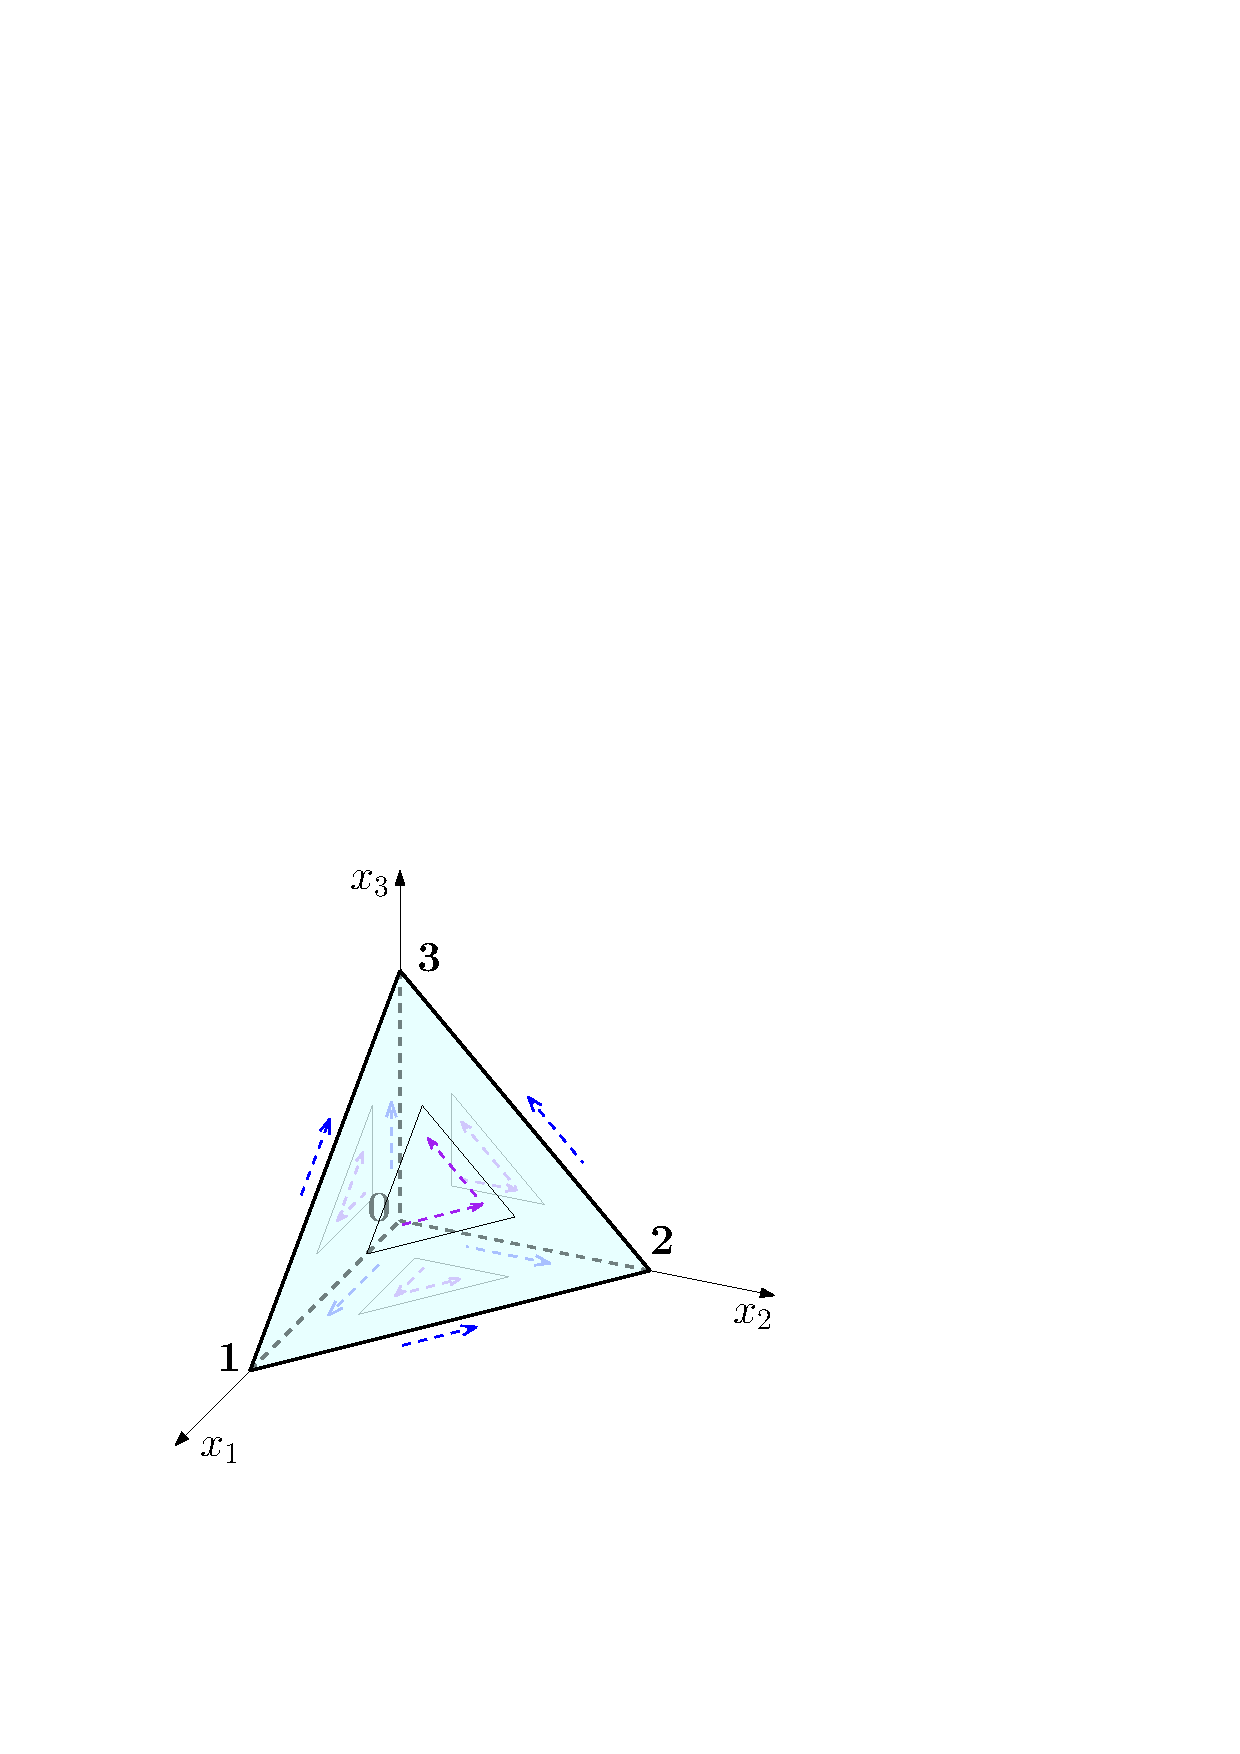
\includegraphics[scale=0.5]{./figures/MasterTetOrientations.pdf}
\caption{Master tetrahedron with numbered vertices \textit{and} local edge and face orientations.}
\label{fig:MasterTetOrientations}
\end{center}
\end{figure}

To construct orientation embedded shape functions for the tetrahedron, it is recommended to have read at least the first part of \S\ref{sec:HexaOrientations}.
The predefined \textit{local} edge and face orientations for the tetrahedron are illustrated in Figure \ref{fig:MasterTetOrientations}.
They represent the $\oo=0$ case.
The task at hand is to find the associated \textit{locally ordered} tuples of affine coordinates representing those local orientations.
As examples take edge 01 and face 012.

Edge 01 is composed of the vertices $v_0$ and $v_1$, which are linked uniquely to $\lambda_0$ and $\lambda_1$ respectively.
The local orientation for edge 01 is represented by the local vertex-ordering $v_0\tdashto v_1$.
As a result, the locally ordered pair for edge 01 is $\vec{\lambda}_{01}=(\lambda_0,\lambda_1)$.
It follows that the orientation embedded edge 01 shape functions in $H^1$ with their gradient are
\begin{equation*}
	\phi_i^\mathrm{e}(x)=\phi_i^\E(\sigma_\oo^\E(\vec{\lambda}_{01}(x)))\,,\qquad\quad
		\nabla\phi_i^\mathrm{e}(x)=\nabla\phi_i^\E(\sigma_\oo^\E(\vec{\lambda}_{01}(x)))\,,
\end{equation*}
with $i=2,\ldots,p$.
The same applies to the $H(\mathrm{curl})$ edge 01 shape functions and their curl.
The approach is analogous with any other edge.

Face 012 is composed of the vertices $v_0$, $v_1$ and $v_2$, which are linked to $\lambda_0$, $\lambda_1$ and $\lambda_2$ respectively.
The local orientation for the face is represented by the local vertex-ordering $v_0\tdashto v_1\tdashto v_2$, and as a result the locally ordered triplet for face 012 is $\vec{\lambda}_{012}=(\lambda_0,\lambda_1,\lambda_2)$.
Hence, for example the $H^1$ orientation embedded face 012 shape functions with their gradient are
\begin{equation*}
	\phi_{ij}^\mathrm{f}(x)=\phi_{ij}^\Tri(\sigma_\oo^\Tri(\vec{\lambda}_{012}(x)))\,,\qquad\quad
		\nabla\phi_{ij}^\mathrm{f}(x)=\nabla\phi_{ij}^\Tri(\sigma_\oo^\Tri(\vec{\lambda}_{012}(x)))\,,
\end{equation*}
with $i\geq2$, $j\geq1$ and $n=i+j=3,\ldots,p$.
The same applies to the $H(\mathrm{curl})$ and $H(\mathrm{div})$ face 012 shape functions and their differential forms.
Naturally, the approach is analogous with any other face.

